\documentclass[11pt]{article}

\usepackage[a4paper,margin=1in]{geometry}
\usepackage{amsmath,amssymb,amsthm}
\usepackage{mathtools}
\usepackage{microtype}
\usepackage{booktabs}
\usepackage{array}
\usepackage{graphicx}
\usepackage{tikz}
\usepackage{pgfplots}
\pgfplotsset{compat=1.18}
\usetikzlibrary{arrows.meta,positioning,calc,shapes.geometric,shapes.misc,fit,backgrounds,decorations.pathreplacing,patterns}
\usepackage[hidelinks]{hyperref}
\usepackage{xcolor}
\usepackage{enumitem}
\usepackage{caption}
\usepackage{tabularx}
\usepackage{verbatim}
\usepackage{url}
\usepackage{algorithm}
\usepackage{algpseudocode}

\definecolor{accent}{HTML}{1f3a93}
\definecolor{accent2}{HTML}{c0392b}
\definecolor{accent3}{HTML}{27ae60}
\definecolor{rule}{HTML}{888888}
\definecolor{lightgray}{HTML}{dcdcdc}

\hypersetup{
  colorlinks=true,
  linkcolor=accent,
  citecolor=accent,
  urlcolor=accent,
}

% Allow extra inter-word stretch in paragraphs containing long unbreakable
% \texttt{} tokens (commit hashes, env-var names, parameter names) so they
% do not produce overfull hboxes.
\emergencystretch=3em
\sloppy

\theoremstyle{plain}
\newtheorem{theorem}{Theorem}
\newtheorem{proposition}[theorem]{Proposition}
\newtheorem{lemma}[theorem]{Lemma}
\theoremstyle{definition}
\newtheorem{definition}[theorem]{Definition}
\newtheorem{remark}[theorem]{Remark}

\newcommand{\bpp}{\mathrm{bpp}}
\newcommand{\kl}{D_{\mathrm{KL}}}
\newcommand{\Linears}{\mathcal{L}}
\newcommand{\Formats}{\mathcal{F}}
\newcommand{\Assignment}{\mathcal{A}}
\newcommand{\R}{\mathbb{R}}
\newcommand{\E}{\mathbb{E}}

\title{\bfseries PrismaQuant and PrismaSCOUT:\\
       Operational Rate--Distortion for\\
       Mixed-Precision Large Language Model Quantization}

\author{Robert Tand\\
        \textit{Independent Researcher}\\
        \texttt{robert.tand@icloud.com}}

\date{May 2026}

\begin{document}
\maketitle

\begin{abstract}
We describe \textsc{PrismaQuant}, a mixed-precision quantization pipeline for
large language models, and \textsc{PrismaSCOUT}, the search-and-select algorithm
at its core. Mixed-precision allocation is conventionally posed as a
constrained discrete optimization in which a per-Linear surrogate cost
$\sum_i u_i(f_i)$ is minimized over format assignments under a total-bit budget.
We argue that this formulation is structurally biased on modern transformers:
the true joint quantization error is non-additive across layers, and surrogate
ranks reliably overshoot when many flips are committed at once. We therefore
decouple \emph{candidate generation} from \emph{candidate selection}. Surrogate
costs propose discrete allocations cheaply via a multi-level hierarchy
($L_1$ probe, $L_2$ perturbed-activation fixed point, $L_3$ propagated end-KL);
every assignment that may ship is then gated by a real, end-to-end
Kullback--Leibler divergence measured on a held-out calibration split. Selection
is performed by a validated-frontier kneedle: the bisection samples
$(\bpp,\,\mathrm{KL})$ pairs adaptively, the dominance filter is widened by an
explicit KL noise floor, and the chosen knee is verified by a
leave-one-out stability diagnostic. A monotone coordinate-descent polish
guarantees the shipped assignment is no worse than the chosen frontier point.
On Qwen3.6\nobreakdash-27B, the pipeline produces a 5.31 bits-per-parameter
artifact with held-out KL $0.0151$, replacing a previously shipped 5.50 bpp
artifact at KL $0.0475$ from the same source weights and the same
export-time quantization tricks --- 11\% smaller and 68\% lower KL on the same
calibration. The artifact is published with DOI \texttt{10.57967/hf/8656}
\cite{Tand2026hf}. A subsequent \emph{production-faithful} polish
(Section~\ref{subsec:prodpolish}), in which the polish-time evaluator is
upgraded to use a closer approximation of the per-Linear quantized weight
the exporter ultimately ships --- joint-NVFP4 sibling-coherent input
global scales, GPTQ reconstruction, scale-sweep, and calibrated activation
clip; block-output match remains on the export-only side --- and
the move set is restructured to start from a
low-bpp floor with a small bits-budget creep, drives the polish-time KL
on Qwen3.6\nobreakdash-27B from $0.0151$ at $5.31$~bpp to $0.0054$ at
$5.39$~bpp on a matched 2$\times$128 token calibration. A re-measurement
on the 8$\times$512 token validation split that backs the v1 5.5~bpp
baseline is in flight at the time of writing; the calibration-matched
polish-time signal is the conservative claim until that completes. We also document, in a separate methodology section, several
numerical methods that were proposed and either implemented-but-deprecated or
rejected outright during the design process: Lagrangian
$\lambda$-bisection on the dual gradient, sandwich proximal recalibration,
block-DP over architectural cliques, sparse pairwise QUBO refinement, top-$K$
Hessian-eigenvalue covering, surrogate-only knee selection, and a
single-anchor probe-only knee predictor. We give the principled argument for
each, and the empirical or structural reason it did not become the shipping
path.
\end{abstract}

\section{Introduction}

Post-training quantization has converged on two dominant axes. Per-tensor
methods --- GPTQ \cite{gptq2022}, AutoRound
\cite{autoround2023}, rotation preprocessors, and most
recently ParoQuant \cite{paroquant} --- improve the per-Linear quantization
error of a fixed format. Allocation methods --- HAWQ-V3 \cite{hawqv3}, the
cross-layer-dependency-aware integer-quadratic-programming approach of
CLADO \cite{clado2023}, the cooperative-game CoopQ allocator \cite{coopq},
and the AutoML-style AMQ \cite{amq} --- choose how many bits to spend
where. The two axes are largely orthogonal: an allocator can sit on top
of any per-tensor toolkit and decide which Linears get 16, 8, 4, 3, or 2
bits.

The allocation literature is unified by a recurring observation: per-layer
sensitivity surrogates (diagonal Hessian traces, Fisher MSEs, output-MSEs)
are biased estimators of joint quantization error. The standard remedy is
to model the bias --- pairwise integer-quadratic programming over an
explicit cross-layer dependency model in CLADO \cite{clado2023}, second-order
ILP in HAWQ-V3 \cite{hawqv3}, Shapley-based cooperative-game allocation
in CoopQ \cite{coopq}. We take a different tack.
\emph{Surrogates generate, real measurement selects.} An allocator does not need
a perfect cost model if every candidate it proposes can be cheaply re-scored
end-to-end on a held-out calibration split. Cross-layer interactions and
propagated effects then cease to be quantities one must \emph{model}; they are
quantities one \emph{observes}, automatically, every time a candidate is gated.

This paper reports the design and engineering of a system, named
\textsc{PrismaQuant}, that operationalizes that principle, and the search
algorithm at its core, \textsc{PrismaSCOUT} (\textbf{S}urrogate-\textbf{C}ascaded
\textbf{O}ptimization \textbf{U}nder \textbf{T}radeoff). Three contributions are
new:

\begin{enumerate}[leftmargin=*,itemsep=2pt]
  \item A \textbf{multi-level cost hierarchy} ($L_1, L_2, L_3$) that separates
    cheap proposal from increasingly faithful measurement. $L_2$ is a
    perturbed-activation fixed point that folds inter-layer coupling into the
    activation cache rather than into a closed-form interaction term. $L_3$ is
    a propagated end-KL measurement performed against a target-specific BF16
    paired baseline, lane-batched and tail-amortized so that one $L_3$ pass at
    Qwen-27B scale takes a tractable wall time.
  \item A \textbf{validated-frontier kneedle}: the elbow of the operational
    rate--distortion curve is found on \emph{measured} $(\bpp,\,\mathrm{KL})$
    pairs, not on a surrogate hull. We add a KL noise floor to the dominance
    filter, an adaptive bisection that refines around the current best knee, a
    leave-one-out stability diagnostic, and a strict monotone polish.
  \item A documented \textbf{methodology of rejected detours}. Several
    numerically attractive ideas (sandwich recalibration, $\lambda$-bisection,
    block-DP, sparse pairwise QUBO, top-$K$ Hessian covering, surrogate-only
    knee, probe-only prediction) were proposed during design, some implemented;
    we report the conditions under which each is principled and the empirical
    reasons each was not adopted as the shipping path.
\end{enumerate}

\noindent\textbf{Headline empirical result.} On Qwen3.6\nobreakdash-27B, with
identical source weights and identical export-time per-tensor tricks (GPTQ damp
sweep, scale sweep, block-output match), \textsc{PrismaSCOUT} produces
a 5.31~bpp artifact with held-out KL $0.0151$. The previously published
\textsc{PrismaQuant}~v1 artifact at the same source was 5.50~bpp with held-out
KL $0.0475$ from the same calibration. The new artifact is 11\% smaller and the
held-out KL is 68\% lower. Only the selection routine changed. A second
selection-only upgrade --- the \emph{production-faithful} polish of
Section~\ref{subsec:prodpolish}, which evaluates candidate flips on a
closer approximation of the per-Linear weight the exporter will ship
rather than on RTN proxies and sweeps from a low-bpp floor under a small
bits-budget creep --- drops the polish-time KL on the same model from
$0.0151$ at $5.31$~bpp to $0.0054$ at $5.39$~bpp on a matched
$2\!\times\!128$ token calibration. Both numbers come from the
polish-time evaluator on the same calibration split and are
apples-to-apples; a re-measurement on the larger
$8\!\times\!512$ split that backs the v1 5.5~bpp baseline is in flight
and will be the load-bearing claim once it completes.

The paper is organized as follows. Section~\ref{sec:related} gives background
and related work. Section~\ref{sec:theory} sets up the theoretical framework:
the rate--distortion view, the additive surrogate failure mode, the cost
hierarchy, the kneedle. Section~\ref{sec:algorithm} states the algorithm.
Section~\ref{sec:rejected} is a deliberate methodology section on the numerical
detours we considered and rejected. Section~\ref{sec:engineering} reports the
engineering work that made the measurement loop tractable.
Section~\ref{sec:results} reports empirical results on Qwen3.6-4B and
Qwen3.6-27B, including an honest accounting of the tool-eval-bench delta.
Section~\ref{sec:discussion} discusses limitations.

\section{Background and Related Work}\label{sec:related}

\paragraph{Per-tensor quantization.} GPTQ \cite{gptq2022} is the workhorse
weight-only quantizer for transformers, posed as Hessian-weighted least squares
over reconstruction error. AutoRound \cite{autoround2023} sign-rounds via
signSGD. Rotation preprocessors transform weight matrices to reduce outlier
counts before integer quantization. These methods take a single matrix and a
fixed format and produce a high-quality quantized version of that matrix; they
do not decide \emph{which} matrix gets which format.

\paragraph{Mixed-precision allocation.} HAWQ-V3 \cite{hawqv3} formulates
mixed-precision quantization as an integer linear program over per-layer
sensitivity (second-order Hessian information) and dyadic arithmetic
constraints. CLADO \cite{clado2023} extends this with an explicit
cross-layer dependency: pairwise quantization-error coupling is measured
on a small data subset and the bit-allocation problem is solved as an
integer quadratic program in seconds, rather than approximated additively
across layers. Recent allocation work for LLMs includes
CoopQ \cite{coopq}, which models layers as a cooperative game and uses a
Shapley-based progressive allocator to capture inter-layer interaction, and
AMQ \cite{amq}, which applies AutoML-style search over per-layer
weight-only bit-widths. Surveys of the broader mixed-precision space have
appeared as the field has matured \cite{mpq_survey}, and recent iterative
allocators include IterQuant \cite{iterquant2026}. The geometric view of
quantization error in \cite{geometry_aware} casts GPTQ as Babai's nearest
plane algorithm and is orthogonal to allocation but informs how a fixed
allocation should round.

\paragraph{Knee detection and operational rate--distortion.} The kneedle
algorithm of \cite{kneedle2011} provides a non-parametric estimator of the
elbow of a tradeoff curve. The closely related operational
rate--distortion (ORD) framing of \cite{ortega1998} establishes that any
discrete-choice rate--distortion problem admits a Lagrangian relaxation whose
solutions trace the lower convex hull of the achievable points. Knees on the
ORD frontier correspond to phase transitions where additional rate buys
disproportionate fidelity. Our work imports the ORD vocabulary --- and avoids
the convex hull, since for mixed-precision LLM quantization the discrete
frontier admits non-convex segments and a $\lambda$-sweep on the dual would
skip them (Section~\ref{subsec:lambda}).

\paragraph{Microscaling formats.} The MXFP4/MXFP6/MXFP8 family is specified by
the OCP microscaling working group \cite{ocp_mx}: 4/6/8-bit elements with
shared FP8 (E8M0 or E5M2) block scales over groups of 32. NVFP4 is NVIDIA's
narrower-group 4-bit format with 16-element FP8 group scales
\cite{nvfp4_blackwell}. NVFP4 weight-only Linears cost $4 + 8/16 = 4.5$\,bpp;
MXFP4 weight-only Linears cost $4 + 8/32 = 4.25$\,bpp. Modern
Blackwell/Hopper GPUs offer first-class kernels for both. Mixed precision in
this paper means an assignment
$\Assignment : \Linears \to \Formats$ where each Linear independently
selects from $\{$BF16, MXFP8, NVFP4, MXFP4, $\dots\}$, subject to
fused-sibling constraints in attention ($q,k,v$) and MoE
($\mathrm{gate\_up},\mathrm{down}$).

\paragraph{Serving.} The artifacts described here are exported to vLLM
\cite{vllm} via the \texttt{compressed-tensors} schema, with format coverage
extending to NVFP4, MXFP8, BF16 passthrough, and (in MoE settings) MXFP4
experts. End-to-end inference uses Blackwell-native kernels.

\subsection{The \textsc{PrismaQuant}~v1 baseline and why it sets a hard bar}\label{subsec:v1}

The artifact \textsc{PrismaSCOUT} replaces was not a weak baseline. The
defining feature of \textsc{PrismaQuant}~v1 is the \emph{mixed-precision
allocator itself}: each Linear in the model independently picks its
serving format from $\{$BF16, MXFP8, NVFP4, MXFP4, source-passthrough$\}$
under a global bits-per-parameter budget, rather than every Linear
sharing one quantization scheme as in single-format methods like GPTQ
\cite{gptq2022}. A tuned per-tensor toolkit runs
\emph{under} whatever format the allocator picks for a given Linear; the
allocator decides where bits should be spent. v1 is worth describing in
its own right both because PrismaSCOUT inherits it wholesale (only the
selection routine changed in the head-to-head comparison of
Table~\ref{tab:27b_headline}) and because understanding what v1 already
captures clarifies which residual is left for joint-allocation methods to
attack.

\paragraph{The mixed-precision allocator.} For each Linear $i$ in the
model, v1 enumerates a candidate menu
$\Formats_i \subseteq \{$BF16, MXFP8, NVFP4, MXFP4, source-passthrough$\}$
filtered by serving-time constraints (MXFP8 tile alignment for the
target kernel, FlashInfer masks, source-dtype eligibility for
passthrough), and assigns each candidate a per-Linear cost
$u_i^{(1)}(f)$ from a HAWQ-style \cite{hawqv3} sensitivity probe fed by
a multi-chunk empirical-Fisher accumulator. A multi-choice knapsack DP
\[
  \min_{\Assignment}\;\sum_i u_i^{(1)}(\Assignment_i) \quad
  \text{s.t.}\quad \sum_i b_i(\Assignment_i)\,n_i \le B \cdot \sum_i n_i
\]
selects one format per Linear under the bits-per-parameter budget $B$,
where $b_i(f)$ is the bit count for Linear $i$ at format $f$ and $n_i$
is its parameter count. Fused-sibling coherence (q/k/v in attention,
$\mathrm{gate\_up}$/$\mathrm{down}$ in MoE) is enforced natively by
grouping siblings into refinement units that enumerate only joint
sibling-coherent format combinations; joint-input-global-scale handling
for fused attention is folded into the DP's transition costs. The
output is a heterogeneous per-Linear assignment that may, for example,
keep the highest-sensitivity attention output projection in BF16, the
medium-sensitivity gate/up projections in MXFP8, the bulk dense MLPs
in NVFP4, and (for native-FP8 source architectures) the down-projection
verbatim from the source. This per-Linear heterogeneity is the
operative quality lever: the shipped v1 Qwen-3.6 27B 5.5 bpp artifact,
for example, mixes BF16, MXFP8, and NVFP4 Linears within a single
model (the vLLM serve dispatches all three kernels at load time) ---
a distribution no single-format method can produce.

\paragraph{The per-tensor toolkit.} For each Linear, after the
allocator has picked its format, v1 composes:

\begin{itemize}[leftmargin=*,itemsep=2pt]
  \item \textbf{Per-layer GPTQ} \cite{gptq2022}, the workhorse
    Hessian-weighted least-squares rounding. v1 ships an adaptive
    \emph{damp probe} (commit \texttt{0cbaddb}) that tries multiple
    Hessian damping coefficients per Linear and picks the lowest measured
    output MSE; a \emph{batched-NVFP4} fast path (commit
    \texttt{f57d960}) processes Linear groups together.
  \item \textbf{Scale sweep} (commit \texttt{7884536}) --- a per-tensor
    scale-factor search that minimizes the post-quantization output MSE
    of each Linear, executed inside the export hot path.
  \item \textbf{Block-output matching} (commits \texttt{9ef0a05},
    \texttt{a6c0cf6}, \texttt{b12f96b}) --- after per-Linear quantization,
    a block-level optimization that re-tunes a subset of parameters so
    that the \emph{block} output matches the BF16 reference, not just the
    individual Linear outputs.
  \item \textbf{Source passthrough} (commits \texttt{705fbcd},
    \texttt{0bf4146}) --- when the source checkpoint is already at a
    serving-compatible precision, the allocator may pick a verbatim
    copy of the source codes and scales rather than re-quantizing; the
    dequant view back to BF16 is lossless, so the per-Linear
    $\Delta\mathrm{loss}$ is exactly zero. This is important for
    native low-precision source architectures (MiniMax, DeepSeek-class)
    where re-quantization can only lose information.
  \item \textbf{Activation clipping and FP32 activation cache}
    (commit \texttt{a5d13db}) --- wins the cost-step vs.\ activation
    quantization tradeoff for formats that benefit from clipped
    activations.
\end{itemize}

The whole pipeline (probe $\to$ allocator $\to$ per-tensor refinement
$\to$ export) runs end-to-end on a UMA host with bounded memory.

\paragraph{Why this works as well as it does.} The combination divides
the quantization problem cleanly into two layers. The mixed-precision
allocator solves the \emph{global} question --- which Linears tolerate
$4$-bit storage and which need $8$ or $16$ --- and the per-tensor
toolkit solves the \emph{local} question --- given a chosen format,
what is the lowest-error rounding for this specific weight matrix. Each
per-tensor component attacks one term of the per-Linear quadratic
$\tfrac12 \langle H_i, (W_i - \hat W_i)^2 \rangle$: GPTQ minimizes
$\langle H_i, (W_i - \hat W_i)^2 \rangle$ under the chosen format;
scale sweep tunes the per-tensor scale to minimize the
remaining error; block-output match closes the gap to the
\emph{block-level} reference, absorbing some of the inter-Linear
coupling without an explicit cross-layer cost model. The HAWQ-style
allocator then spends bits on the Linears whose local quadratic has
the largest top eigenvalue. Each technique is narrow, principled, and
composable inside its own layer; together they extract most of the
per-Linear quantization headroom \emph{conditional on} a fixed
allocation.

The empirical evidence that this pipeline is strong is the community
adoption: the public Qwen-3.6 27B, Qwen-3.5 122B-A10B, Qwen-3.6 35B-A3B,
Mistral-Medium-3.5, MiniMax-M2.7, Gemma-4-31B, and DSv4-Flash
\textsc{PrismaQuant}~v1 artifacts have together accumulated over
$60{,}000$ downloads on Hugging Face in their first weeks of release,
across a heterogeneous set of source architectures (dense, MoE, and
native-FP8). v1 is a competitive shipping default in absolute terms.

\paragraph{The stacking-interference failure mode.} Per-tensor
techniques are conventionally treated as additive in single-format
quantization, and on the per-Linear metrics each pass optimizes against
this composition is empirically robust. In a mixed-precision setting it
is not. Each pass operates on the activation distribution as modified
by the previous pass, and the per-Linear cost models the passes consume
are decoupled from the format choices the allocator eventually makes
for upstream Linears. Pairs of individually validated wins can therefore
interfere when stacked: an internal audit confirmed a recipe with all
four wins enabled lost roughly half the gain of activation-clipping
applied alone, with the do-no-harm gate reverting clip-improved Linears
because its cached MSE comparison ran on the unclipped activation
distribution while the upstream pass had optimized under the clipped
one. The per-Linear ``do no harm'' gate (commit \texttt{ed9c60c}) is the
direct band-aid: after GPTQ + scale-sweep, compare against pure RTN
on the cached activations and revert that Linear if RTN beats the
post-pass weight. Both observations are artifacts of the same
structural property --- per-tensor wins that modify the activation
distribution do not propagate that modification forward into the cost
models the downstream wins consume, so cumulative recipes are not, in
general, the composition of their individually-validated parts.

\paragraph{What v1 leaves on the table.} The systematic gap v1 cannot
close from the per-layer view is the joint-allocation question:
``which Linear should pay an extra bit?'' Per-layer sensitivity
correlates with end-KL impact but does not predict it perfectly,
because end-KL depends on how a Linear's quantization error
\emph{propagates} downstream, and propagation is sensitive to the
formats chosen for upstream Linears. v1's HAWQ-style allocator
overspends on Linears with high local sensitivity but modest
downstream impact, and underspends on Linears with low local
sensitivity but errors that compound through later attention. The
stacking-interference failure mode of the previous paragraph is the
mirror image of this gap on the per-tensor side: when upstream
optimization decisions are not propagated into the cost model that
downstream optimizations consume, the resulting cumulative recipe is
not the composition of its individually-validated parts. PrismaSCOUT
does not change a single per-Linear technique; it changes the
allocator from \emph{additive surrogate cost} to \emph{validated end-KL
on real assignments}, and it gates every shipping decision on a held-out
KL measurement. The real-KL gate is also what catches the
stacking-interference failure mode end-to-end --- if a recipe stack
quietly regresses on real KL, no DP rearrangement of the per-Linear
costs hides that fact. The Qwen3.6-27B head-to-head in
Table~\ref{tab:27b_headline} is the empirical statement of this
relationship: the per-Linear toolkit is held fixed, only the selection
routine changes, and the resulting artifact is $11\%$ smaller and
$68\%$ lower in held-out KL. The remaining headroom is at the joint
level, which is where the rest of this paper goes.

\section{Theoretical Framework}\label{sec:theory}

\subsection{The shipping criterion}

Let $p_\theta$ denote the full-precision teacher model with parameters $\theta$
and $p_{\hat\theta}$ a quantized variant with weights $\hat\theta = Q_\Assignment(\theta)$
under format assignment $\Assignment$. Given a calibration distribution
$\mathcal{D}$ over input prefixes $x_{1:t}$, the operational quality of
$\Assignment$ is

\begin{equation}\label{eq:kl}
  \kl(\Assignment) \;=\;
   \frac{1}{N\,T}\sum_{n=1}^{N}\sum_{t=1}^{T_n}
   \kl\!\left[\,p_\theta(\,\cdot \mid x^{(n)}_{1:t})\,\big\|\,
                p_{\hat\theta}(\,\cdot \mid x^{(n)}_{1:t})\,\right],
\end{equation}

\noindent that is, the per-token KL between teacher and quantized
model averaged over $T = \sum_n T_n$ non-padding positions in $N$
calibration prefixes.

KL is the natural objective for ``does the quantized model behave like the
teacher?'' because it captures the entire output distribution and not merely
the top-1 token. Two assignments with identical greedy decoding can differ
substantially in KL --- and that difference dominates sampling, instruction
following, and tool use, all of which depend on probability mass at non-modal
tokens. Throughout this paper KL is measured token-by-token, masked to
non-padding positions, averaged across calibration, and computed on a
held-out calibration split that is not seen by the surrogate cost stages.

\subsection{The additive-surrogate failure mode}

A natural objective for allocation is the additive sum of per-Linear costs

\begin{equation}\label{eq:additive}
  U_{\mathrm{add}}(\Assignment) \;=\; \sum_{i \in \Linears} u_i(\Assignment_i)
\end{equation}

where $u_i(f)$ is the local cost of using format $f$ at Linear $i$, holding
all other Linears at some reference assignment $\Assignment^{(\mathrm{ref})}$.
The diagonal Hessian formulation
$u_i(f) = \mathrm{Tr}(H_i)\cdot \mathrm{MSE}_i(f)$ used by HAWQ
\cite{hawqv3} is one example; output-MSE under fixed activation context is
another. \emph{For any choice of $u_i$ that holds $\Assignment_{-i}$ fixed,
$U_{\mathrm{add}}$ is a first-order Taylor expansion of $\kl(\Assignment)$
centered at $\Assignment^{(\mathrm{ref})}$.} A constrained minimization of
$U_{\mathrm{add}}$ subject to a bit budget $B$ via additive multi-choice
knapsack DP greedily flips many Linears at once and routinely steps outside
the trust region of the linear approximation. Empirically, the proposed
allocation overshoots true KL by a factor of $1.3$--$1.5$ on the
configurations we measured; a 0.10 unit predicted decrease can produce a 0.08
unit measured \emph{increase}.

This is the structural hazard the rest of the paper is built around.
Figure~\ref{fig:nonadditivity} sketches the geometry.

\begin{figure}[t]
\centering
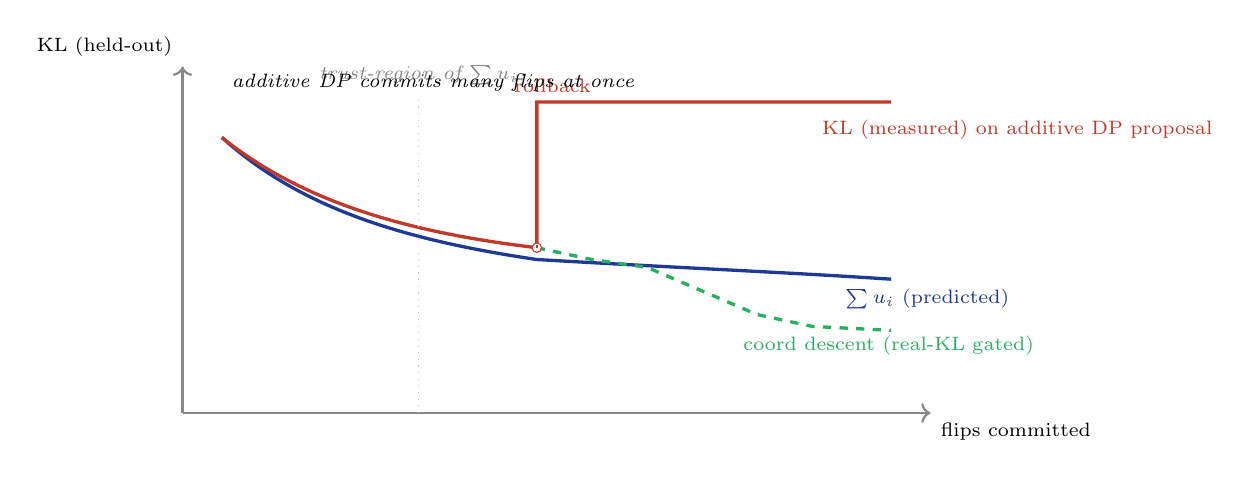
\begin{tikzpicture}[
  every node/.style={font=\small},
  axis/.style={->, thick, draw=rule}
]
  % Frame
  \def\xa{0}\def\xb{9.5}\def\ya{0}\def\yb{4.4}
  \draw[axis] (\xa,\ya) -- (\xb,\ya) node[below right, font=\scriptsize]{flips committed};
  \draw[axis] (\xa,\ya) -- (\xa,\yb) node[above left, font=\scriptsize]{KL (held-out)};

  % Predicted (additive surrogate) trace — monotone decrease with flips
  \draw[draw=accent, very thick]
    (0.5, 3.5) .. controls (1.5,2.6) and (2.8,2.2) ..
    (4.5, 1.95) .. controls (6.2,1.85) and (7.8,1.78) ..
    (9.0, 1.7);
  \node[font=\scriptsize, text=accent, anchor=west] at (8.3, 1.45) {$\sum u_i$ (predicted)};

  % Measured KL trace — initially follows, then explodes upward at many-flip step
  \draw[draw=accent2, very thick]
    (0.5, 3.5) .. controls (1.5,2.7) and (2.8,2.3) ..
    (4.5, 2.1)
    -- (4.5, 3.95)
    -- (9.0, 3.95);
  \node[font=\scriptsize, text=accent2, anchor=west] at (8.0, 3.6)
    {KL (measured) on additive DP proposal};

  % Coord descent (monotone) trace from rollback point
  \draw[draw=accent3, very thick, dashed]
    (4.5, 2.1) -- (5.2, 1.95) -- (5.9, 1.85) --
    (6.6, 1.55) -- (7.3, 1.25) -- (8.0, 1.10) -- (9.0, 1.05);
  \node[font=\scriptsize, text=accent3, anchor=west] at (7.0, 0.85)
    {coord descent (real-KL gated)};

  % Rollback marker
  \node[circle, draw=accent2, fill=white, inner sep=1.2pt] at (4.5, 2.1) {};
  \draw[draw=accent2, dotted, thick] (4.5, 2.1) -- (4.5, 3.95);
  \node[anchor=south, font=\scriptsize, text=accent2] at (4.7, 3.95) {rollback};

  % Trust-region annotation
  \draw[draw=rule!50, dotted] (3.0, 0) -- (3.0, 4.0);
  \node[anchor=south, font=\scriptsize\itshape, text=rule] at (3.0, 4.05)
    {trust-region of $\sum u_i$};

  % Caption-internal labels
  \node[font=\scriptsize, anchor=west] at (0.5, 4.2)
    {\itshape additive DP commits many flips at once};
\end{tikzpicture}
\caption{The non-additivity overshoot. The additive surrogate
$U_{\mathrm{add}} = \sum u_i$ predicts a monotone KL decrease as flips
accumulate (blue). The real, measured held-out KL agrees with the surrogate
inside the trust region of the local Taylor expansion, but diverges
sharply when many flips are committed at once (red). The validated-frontier
gate detects the regression and rolls back to the prior assignment;
coord-descent then makes single-Linear flips, each gated on real KL
(green dashed), and is monotone non-increasing by construction.}
\label{fig:nonadditivity}
\end{figure}


\subsection{Surrogates generate, real measurement selects}

The remedy adopted in \textsc{PrismaSCOUT} is to use $U_{\mathrm{add}}$ purely
as a \emph{candidate generator} and to select from generated candidates by
real, end-to-end measurement of $\kl(\Assignment)$ on a held-out calibration
split. The objective inequality
\[
  U_{\mathrm{add}}(\Assignment) \le U_{\mathrm{add}}(\Assignment') \quad
  \not\Longrightarrow \quad \kl(\Assignment) \le \kl(\Assignment')
\]
fails on average for many-flip moves. The substitute property
\[
  \kl(\Assignment) \le \kl(\Assignment')\quad\text{(measured on held-out)}
\]
is observable for any pair we are willing to materialize and forward through
the model. The cost of \emph{making} that observation is what determines
whether the surrogates-generate paradigm is practical at LLM scale, which is
where the cost hierarchy enters.

\subsection{The cost hierarchy}\label{subsec:hierarchy}

\textsc{PrismaSCOUT} runs three escalating cost models on the same problem
(Figure~\ref{fig:cost_hierarchy}).

\begin{description}[leftmargin=2em,style=nextline]
  \item[$L_1$ probe ($\sim$\,seconds per Linear).] A coarse per-matrix
    surrogate produced by a multi-chunk probe pass that accumulates an
    empirical Fisher trace $\mathrm{Tr}(\hat H_i)$ alongside per-format
    output perturbation \cite{prismaquant}. The allocator's preferred
    cost is $u_i^{(1)}(f) = \tfrac12 \langle \hat H_i^{\mathrm{full}},
    (W_i - Q_f(W_i))^2 \rangle$, the second-order $\Delta\mathrm{loss}$
    proxy when a per-weight Hessian detail tensor is available; otherwise
    it falls back through measured local output MSE
    $\mathrm{MSE}\!\big(W_i X^{(0)},\, Q_f(W_i)\,X^{(0)}\big)$ and finally
    $\mathrm{Tr}(\hat H_i)\cdot \mathrm{MSE}_i^{\mathrm{w}}(f)$, the
    Fisher-trace-weighted weight-MSE scalar (\texttt{measure\_quant\_cost.py}).
    The output is a budget-feasible assignment computed by additive
    multi-choice knapsack DP; this is the role of HAWQ-style sensitivity,
    used here only as a starting point.
  \item[$L_2$ perturbed-X fixed point ($\sim$\,minutes).] A more careful
    per-Linear measurement that captures the activation distribution
    \emph{under the current assignment} rather than under BF16. We install
    pre-quantization activation hooks on the model under $\Assignment^{(k)}$,
    forward calibration tokens, and cache the resulting activations
    $X^{(k)}$. We then measure
    \[
      u_i^{(2)}(f) \;=\; \mathrm{MSE}\!\left(W_i\,X^{(k)},\; Q_f(W_i)\,Q_f^{\mathrm{act}}(X^{(k)})\right),
    \]
    where $Q_f^{\mathrm{act}}(\cdot)$ is the activation quantize-dequantize
    of the format under measurement (identity for weight-only formats; the
    matched activation quantizer for formats with native activation
    quantization), and the resulting scalar is fed through the same
    $\Delta\mathrm{loss}$/Fisher-trace cost machinery as $L_1$. The DP solves
    under $u^{(2)}$, producing $\Assignment^{(k+1)}$. The fixed-point
    iteration $\Assignment \to X \to u^{(2)} \to \Assignment$ typically
    converges in $2$--$3$ iterations on the models we have measured.
    Convergence is declared when the weighted-Hamming flip ratio
    \[
      h^{(k)} \;=\;
      \frac{\sum_{i:\,\Assignment^{(k+1)}_i \neq \Assignment^{(k)}_i} n_i}{\sum_i n_i}
    \]
    (parameter-count weighted, with $n_i$ the parameter count of Linear
    $i$) falls below \texttt{convergence-frac} (default $0.01$).
    Inter-layer coupling enters through the activation cache:
    late-layer activations under a low-bit early-layer assignment differ
    from BF16 activations, and the per-Linear cost adapts.
  \item[$L_3$ propagated cost ($\sim$\,tens of minutes).] An end-KL
    measurement against a \emph{target-specific BF16 paired baseline}. For
    each candidate $(\mathrm{Linear}\;\ell,\,\mathrm{format}\;f)$, we run two
    forwards: a baseline lane in which Linear $\ell$ is BF16 and every other
    Linear is at its $L_2$ assignment, and a candidate lane in which Linear
    $\ell$ uses format $f$. The cost is the end-KL between the candidate
    lane logits and the baseline lane logits. Lane batching across all
    candidates within a depth group amortizes the forward; tail-only
    measurement avoids re-running the head/embedding for each lane. The
    output is a per-(Linear, format) end-KL table $u^{(3)}_i(f)$ that the
    final DP consumes.
\end{description}

\begin{figure}[t]
\centering
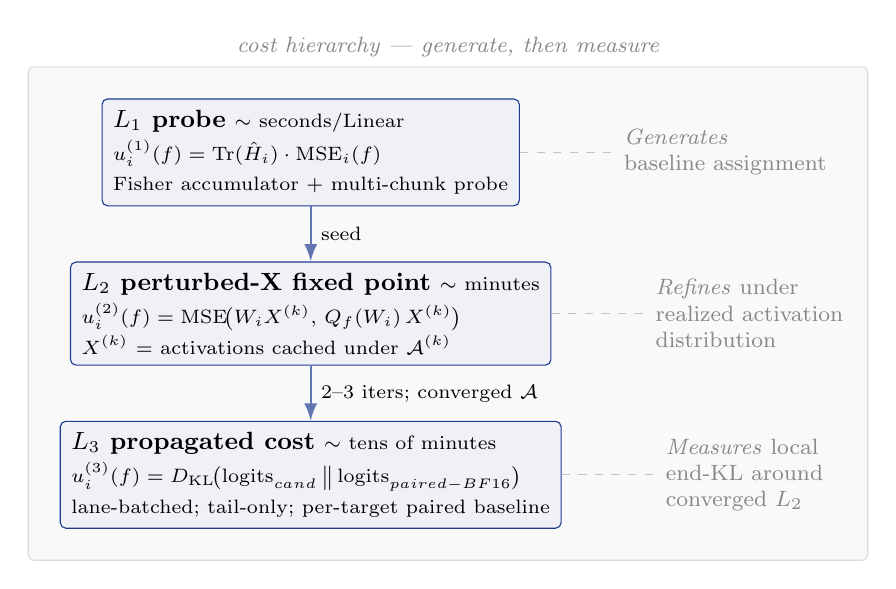
\begin{tikzpicture}[
  every node/.style={font=\small},
  level/.style={draw=accent, fill=accent!7, rounded corners=2pt,
                minimum width=46mm, minimum height=12mm,
                align=left, inner sep=4pt},
  cost/.style={font=\scriptsize, text=accent},
  arr/.style={-{Latex[length=2.2mm]}, thick, draw=accent!70}
]
  \node[level] (l1)
    {{\bfseries $L_1$ probe} \hfill {\scriptsize $\sim$ seconds/Linear} \\[1pt]
     \scriptsize $u_i^{(1)}(f) = \mathrm{Tr}(\hat H_i)\cdot \mathrm{MSE}_i(f)$ \\
     \scriptsize Fisher accumulator + multi-chunk probe};

  \node[level, below=7mm of l1] (l2)
    {{\bfseries $L_2$ perturbed-X fixed point} \hfill {\scriptsize $\sim$ minutes} \\[1pt]
     \scriptsize $u_i^{(2)}(f) = \mathrm{MSE}\!\big(W_i X^{(k)},\, Q_f(W_i)\,X^{(k)}\big)$ \\
     \scriptsize $X^{(k)}$ = activations cached under $\Assignment^{(k)}$};

  \node[level, below=7mm of l2] (l3)
    {{\bfseries $L_3$ propagated cost} \hfill {\scriptsize $\sim$ tens of minutes} \\[1pt]
     \scriptsize $u_i^{(3)}(f) = \kl\!\big(\mathrm{logits}_{cand}\,\big\|\,\mathrm{logits}_{paired-BF16}\big)$ \\
     \scriptsize lane-batched; tail-only; per-target paired baseline};

  \node[right=12mm of l1, font=\footnotesize, align=left, text=rule] (l1n)
    {\emph{Generates}\\ baseline assignment};
  \node[right=12mm of l2, font=\footnotesize, align=left, text=rule] (l2n)
    {\emph{Refines} under\\ realized activation\\ distribution};
  \node[right=12mm of l3, font=\footnotesize, align=left, text=rule] (l3n)
    {\emph{Measures} local\\ end-KL around\\ converged $L_2$};

  \draw[arr] (l1) -- node[right, midway, font=\scriptsize]{seed} (l2);
  \draw[arr] (l2) -- node[right, midway, font=\scriptsize]{$2$--$3$ iters; converged $\Assignment$} (l3);

  \draw[draw=rule!50, dashed] (l1.east) -- (l1n.west);
  \draw[draw=rule!50, dashed] (l2.east) -- (l2n.west);
  \draw[draw=rule!50, dashed] (l3.east) -- (l3n.west);

  \begin{scope}[on background layer]
    \node[draw=rule!30, fill=rule!5, rounded corners=2pt,
          fit=(l1)(l2)(l3)(l3n)(l1n),
          inner sep=4mm,
          label={[font=\footnotesize\itshape, text=rule]above:cost hierarchy --- generate, then measure}] {};
  \end{scope}
\end{tikzpicture}
\caption{The three-level cost hierarchy. $L_1$ and $L_2$ are surrogate cost
models used for candidate generation; $L_3$ is a real, end-to-end
KL-divergence measurement against a target-specific paired baseline. The
$L_2$ fixed point folds inter-layer coupling into the activation cache so
that the per-Linear surrogate adapts to the realized assignment.}
\label{fig:cost_hierarchy}
\end{figure}


The three levels are wired in cascade: $L_1$ proposes, $L_2$ refines under the
proposed activation distribution, $L_3$ measures the end-effect locally
around the converged $L_2$ assignment.
$L_3$ semantics differ from $L_1$ and $L_2$ in a load-bearing way: $L_3$
\emph{is} an end-KL measurement, just one whose paired baseline freezes the
context outside the target Linear at the converged $L_2$ assignment rather
than at BF16. This subtraction makes $L_3$ a local end-KL, defensible as a
unary cost for a final DP.

\subsection{The validated-frontier kneedle}\label{subsec:kneedle}

The validated-frontier construction is sketched in
Figure~\ref{fig:kneedle}. After the cost hierarchy generates a set of
candidate assignments
$\{\Assignment^{(j)}\}$ at multiple budgets, each candidate is materialized,
forwarded against the held-out calibration split, and assigned a measured pair
$(\bpp(\Assignment^{(j)}),\,\kl(\Assignment^{(j)}))$. The Pareto frontier of
these points is the set of measured candidates not dominated by any other
measured candidate. The dominance filter is widened by an explicit KL noise
floor $\eta$:

\begin{definition}[$\eta$-dominance]
$\Assignment$ $\eta$-dominates $\Assignment'$ if
$\bpp(\Assignment) \le \bpp(\Assignment')$ and
$\kl(\Assignment) + \eta < \kl(\Assignment')$.
\end{definition}

This avoids spurious points on the frontier created by KL measurement noise
within $\eta$ of a competing point. The kneedle is then computed on the
$\eta$-non-dominated frontier as the point of maximum perpendicular distance
to the secant joining the frontier endpoints, after standard min-max
normalization of both axes. Concretely, with normalized
$(\tilde x_i, \tilde y_i)$ on the frontier in increasing-$\bpp$ order, and
$\tilde y$ replaced by $1 - \tilde y$ so the curve is increasing,

\begin{equation}\label{eq:kneedle}
  i^\star \;=\; \arg\max_i\;
  \frac{\big| (\tilde y_n - \tilde y_1)\tilde x_i - (\tilde x_n - \tilde x_1)\tilde y_i + \tilde x_n \tilde y_1 - \tilde y_n \tilde x_1 \big|}{\sqrt{(\tilde y_n - \tilde y_1)^2 + (\tilde x_n - \tilde x_1)^2}}.
\end{equation}

The kneedle is endpoint-fallback: if the maximum-perpendicular point is one of
the two endpoints (a near-linear frontier), the central point is used instead
and a warning is emitted. Adaptive bisection refines the frontier by
evaluating the midpoint of the largest gap adjacent to the current best knee
until either $|\bpp_R - \bpp_L| < \tau$ or the evaluation budget is reached.

\begin{figure}[t]
\centering
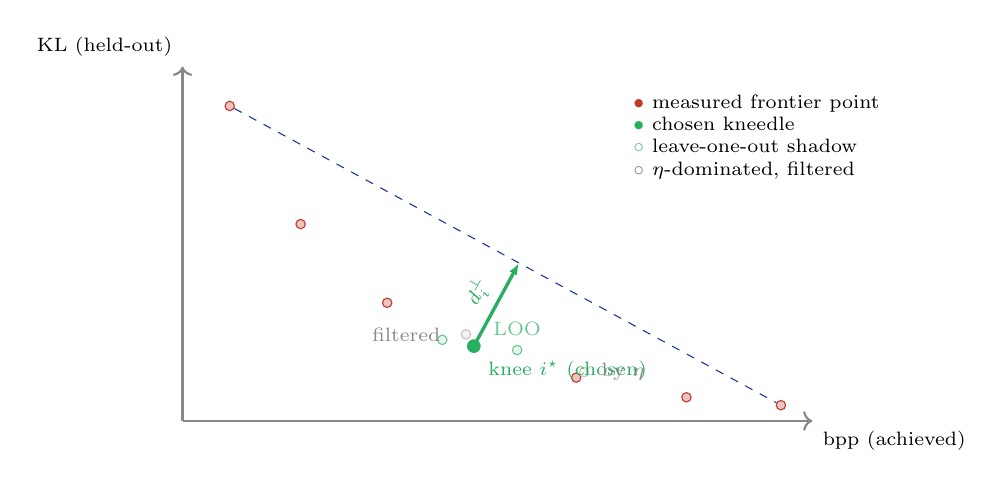
\begin{tikzpicture}[
  every node/.style={font=\small},
  pt/.style={circle, draw=accent2, fill=accent2!30, inner sep=1.2pt},
  filtered/.style={circle, draw=rule!50, fill=rule!10, inner sep=1.2pt},
  knee/.style={circle, draw=accent3, fill=accent3, inner sep=1.6pt},
  loo/.style={circle, draw=accent3!70, fill=accent3!10, inner sep=1.2pt},
  axis/.style={->, thick, draw=rule}
]
  \def\xa{0}\def\xb{8.0}\def\ya{0}\def\yb{4.5}
  \draw[axis] (\xa,\ya) -- (\xb,\ya) node[below right, font=\scriptsize]{$\bpp$ (achieved)};
  \draw[axis] (\xa,\ya) -- (\xa,\yb) node[above left, font=\scriptsize]{KL (held-out)};

  % Pareto-frontier-shaped points
  \node[pt] (P1) at (0.6, 4.0) {};
  \node[pt] (P2) at (1.5, 2.5) {};
  \node[pt] (P3) at (2.6, 1.5) {};
  \node[pt] (P4) at (3.7, 0.95) {}; % near-knee
  \node[pt] (P5) at (5.0, 0.55) {};
  \node[pt] (P6) at (6.4, 0.30) {};
  \node[pt] (P7) at (7.6, 0.20) {};

  % Filtered (eta-dominated) point — same bpp neighborhood, slightly worse KL
  \node[filtered] (F1) at (3.6, 1.10) {};
  \node[filtered] (F2) at (5.1, 0.62) {};

  % Secant
  \draw[draw=accent, dashed] (P1) -- (P7);

  % Knee (highlight P4)
  \node[knee, label={[font=\scriptsize, text=accent3]below right:knee $i^\star$ (chosen)}] at (P4) {};

  % Perpendicular drop from knee to secant
  \coordinate (Pfoot) at ($ (P1)!(P4)!(P7) $);
  \draw[draw=accent3, very thick, -{Latex[length=1.5mm]}] (P4) -- (Pfoot)
    node[midway, sloped, above, font=\scriptsize, text=accent3]{$d^\perp_i$};

  % LOO shadow knees
  \node[loo, label={[font=\scriptsize, text=accent3!70]above:LOO}] at ($(P4)+(0.55,-0.05)$) {};
  \node[loo] at ($(P4)+(-0.40,0.08)$) {};

  % Annotations
  \node[font=\scriptsize, text=rule, anchor=east] at (3.4, 1.10) {filtered};
  \node[font=\scriptsize, text=rule, anchor=west] at (5.2, 0.62) {by $\eta$};

  \node[font=\scriptsize, anchor=west] at (5.6, 3.6)
   {\begin{tabular}{@{}l@{}}
     {\color{accent2}$\bullet$} measured frontier point\\
     {\color{accent3}$\bullet$} chosen kneedle\\
     {\color{accent3!70}$\circ$} leave-one-out shadow\\
     {\color{rule}$\circ$} $\eta$-dominated, filtered
    \end{tabular}};
\end{tikzpicture}
\caption{Validated-frontier kneedle. Each point on the frontier is a
real, end-to-end held-out KL measurement of a materialized candidate
assignment. The dominance filter widens by an explicit KL noise floor
$\eta$. The chosen knee maximizes perpendicular distance to the
endpoint-secant after min-max normalization
(Equation~\ref{eq:kneedle}). The leave-one-out diagnostic re-runs the
kneedle on each subset of size $|F|-1$; if the maximum bpp shift exceeds
tolerance, the search emits an instability warning and records a guarded
fallback knee.}
\label{fig:kneedle}
\end{figure}


\subsection{Leave-one-out stability}\label{subsec:loo}

A frontier with $5$--$7$ points is small enough that the chosen knee can be
brittle. We add a leave-one-out diagnostic: for each frontier point $i$,
remove it and re-run the kneedle (Figure~\ref{fig:loo_stability}). If the
maximum bpp shift across removals exceeds tolerance, or the maximum KL
shift exceeds $\eta$, the search emits an instability warning, and the
artifact metadata records both the chosen knee and a guarded fallback. The
default guard policy when the diagnostic flags instability is
\texttt{best-kl}: replace the geometric kneedle with the lowest measured-KL
frontier point. We do not hard-fail on instability; we record it. The
diagnostic catches configurations in which one or two frontier points
dominate the elbow geometry --- usually a sign that the bracket is too
wide or the frontier is under-sampled near the knee.

\begin{figure}[t]
\centering
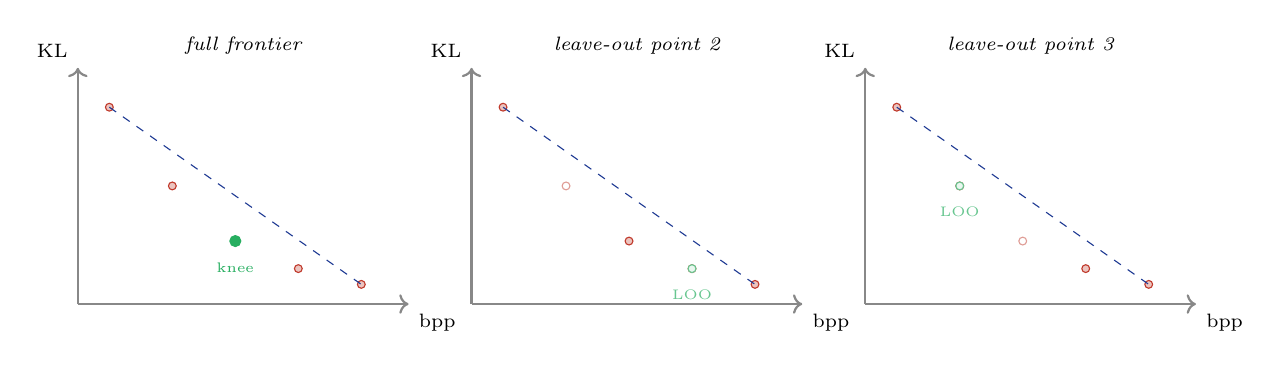
\begin{tikzpicture}[
  every node/.style={font=\scriptsize},
  pt/.style={circle, draw=accent2, fill=accent2!30, inner sep=1.0pt},
  pt_removed/.style={circle, draw=accent2!50, fill=white, inner sep=1.0pt},
  knee_orig/.style={circle, draw=accent3, fill=accent3, inner sep=1.4pt},
  knee_loo/.style={circle, draw=accent3!70, fill=accent3!10, inner sep=1.0pt},
  axis/.style={->, thick, draw=rule}
]

% Three panels side by side: full, leave-one-out (i=2), leave-one-out (i=3)
\foreach \panel/\title/\removed in {0/full frontier/-1, 5/leave-out point 2/2, 10/leave-out point 3/3} {
  \begin{scope}[xshift=\panel cm]
    \draw[axis] (0,0) -- (4.2,0) node[below right]{$\bpp$};
    \draw[axis] (0,0) -- (0,3.0) node[above left]{KL};

    % 5 frontier points
    \pgfmathsetmacro{\xa}{0.4}\pgfmathsetmacro{\ya}{2.5}
    \pgfmathsetmacro{\xb}{1.2}\pgfmathsetmacro{\yb}{1.5}
    \pgfmathsetmacro{\xc}{2.0}\pgfmathsetmacro{\yc}{0.8}  % near-knee
    \pgfmathsetmacro{\xd}{2.8}\pgfmathsetmacro{\yd}{0.45}
    \pgfmathsetmacro{\xe}{3.6}\pgfmathsetmacro{\ye}{0.25}

    % Render points (filled or empty depending on removed)
    \ifnum\removed=2
      \node[pt_removed] at (\xb,\yb) {};
      \node[pt] at (\xa,\ya) {};
      \node[pt] at (\xc,\yc) {};
      \node[pt] at (\xd,\yd) {};
      \node[pt] at (\xe,\ye) {};
    \else
      \ifnum\removed=3
        \node[pt_removed] at (\xc,\yc) {};
        \node[pt] at (\xa,\ya) {};
        \node[pt] at (\xb,\yb) {};
        \node[pt] at (\xd,\yd) {};
        \node[pt] at (\xe,\ye) {};
      \else
        \node[pt] at (\xa,\ya) {};
        \node[pt] at (\xb,\yb) {};
        \node[pt] at (\xc,\yc) {};
        \node[pt] at (\xd,\yd) {};
        \node[pt] at (\xe,\ye) {};
      \fi
    \fi

    % Secant on remaining points
    \ifnum\removed=2
      \draw[draw=accent, dashed] (\xa,\ya) -- (\xe,\ye);
    \else
      \ifnum\removed=3
        \draw[draw=accent, dashed] (\xa,\ya) -- (\xe,\ye);
      \else
        \draw[draw=accent, dashed] (\xa,\ya) -- (\xe,\ye);
      \fi
    \fi

    % Knee marker (different position depending on which is removed)
    \ifnum\removed=2
      % LOO knee shifts slightly
      \node[knee_loo] at (\xd,\yd) {};
      \node[anchor=north, font=\tiny, text=accent3!70] at (\xd,\yd-0.15) {LOO};
    \else
      \ifnum\removed=3
        % Removing the actual knee shifts further
        \node[knee_loo] at (\xb,\yb) {};
        \node[anchor=north, font=\tiny, text=accent3!70] at (\xb,\yb-0.15) {LOO};
      \else
        \node[knee_orig] at (\xc,\yc) {};
        \node[anchor=north, font=\tiny, text=accent3] at (\xc,\yc-0.15) {knee};
      \fi
    \fi

    \node[font=\scriptsize\itshape, anchor=south] at (2.1, 3.05) {\title};
  \end{scope}
}

\end{tikzpicture}
\caption{Leave-one-out kneedle stability. The diagnostic re-runs the
kneedle algorithm on each subset of size $|F|-1$ obtained by removing one
frontier point. If the maximum bpp shift across removals exceeds tolerance,
or the maximum KL shift exceeds the noise floor $\eta$, the search emits
an instability warning and records both the original knee and a guarded
fallback. In the synthetic example shown: removing a non-knee point
(middle) leaves the knee location nearly unchanged; removing the knee point
itself (right) shifts the LOO knee to a neighboring frontier point. A
configuration that produces shifts of the latter type at every removal is
an indication that the bracket is too wide or the frontier is
under-sampled.}
\label{fig:loo_stability}
\end{figure}


\subsection{Coordinate descent as monotone polish}\label{subsec:coord}

The polish trace is illustrated in Figure~\ref{fig:coord_descent}.

The polish does not produce a mathematical discovery; it provides a
contractual guarantee that the shipped assignment cannot be worse than
the chosen frontier point under the polish-time evaluator. We state the
contract formally so that what it covers, and what it does not, is
explicit.

\begin{proposition}[Design guarantee, monotone non-regression of coord-descent polish]\label{prop:monotone}
Fix a calibration prefix set $C$, a deterministic logits evaluator
$\mathcal{E}$ (model class, kernel selection, RNG state, and
quantization rounding mode all held constant), a fused-sibling-coherent
move set $\mathcal{M}$, and a numerical-stability tolerance
$\varepsilon \ge 0$. Write $K(\Assignment) \equiv \kl(\Assignment;\,C,\,\mathcal{E})$
for the KL measured against this fixed pair. Let $\Assignment^{(0)}$ be
the chosen knee assignment with $\kappa_0 = K(\Assignment^{(0)})$. The
coord-descent polish iterates single-refinement-unit flips
$\Assignment^{(t+1)} = \Assignment^{(t)}\!\big[i \to f^\star\big]$
drawn from $\mathcal{M}$ and accepts only flips that satisfy
$K(\Assignment^{(t+1)}) < K(\Assignment^{(t)}) - \varepsilon$. Then the
output assignment $\Assignment^{(\infty)}$ satisfies
$K(\Assignment^{(\infty)}) \le \kappa_0$.
\end{proposition}

\begin{proof}
Each accepted flip strictly decreases $K$ on the fixed $(C, \mathcal{E})$
pair by more than $\varepsilon$; rejected flips leave the assignment
and $K$ unchanged. The sequence $\{K(\Assignment^{(t)})\}$ is monotone
non-increasing.
\end{proof}

The implementation uses $\varepsilon = 10^{-12}$ as a numerical-stability
floor (strict less-than under floating-point roundoff;
\texttt{coordinate\_descent\_polish} in
\texttt{iterate\_perturbed\_allocation.py}). The proof is one line; the
load-bearing content is the proposition's scope.

\begin{remark}\label{rem:monotone_scope}
Proposition~\ref{prop:monotone} guarantees non-regression on the
calibration prefix set, the evaluator, and the move set fixed at polish
time. It does not extend to (i) a different held-out calibration set,
(ii) a different evaluator (e.g.\ post-export inference engine,
alternate kernel choice), or (iii) post-polish assignment mutation
outside $\mathcal{M}$ (e.g.\ exporter-side fused-sibling rewrites,
format coercions imposed by serving constraints). The shipped artifact
is therefore re-validated end-to-end after export to bound the residual
divergence between the polish-time evaluator and the production
inference engine.
\end{remark}

The operationally important point is that the polish does not need a
cost model. It does not need to predict the change in KL; it measures
it. The flip ranking comes from $L_3$ unary costs (cheap), the
acceptance criterion is real KL on held-out (slow but rare). On Qwen3.6-4B at
the 4.5~bpp anchor, coord descent committed 6 flips out of 101 attempts and
moved KL from $0.371$ (post-$L_2$) to $0.245$, a $34\%$ improvement. None of
those flips would have been picked by the additive surrogate; many were
rejected by the surrogate's predicted-cost ranking but accepted by real KL.

\begin{figure}[t]
\centering
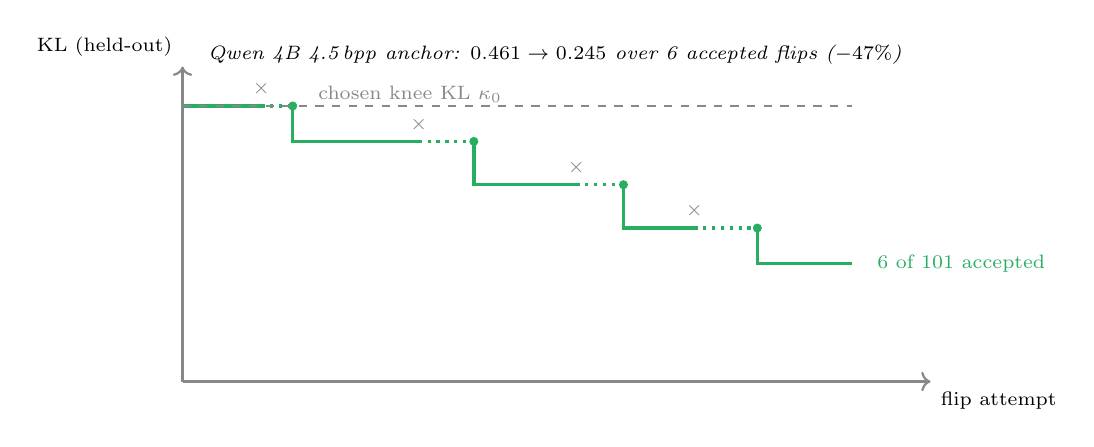
\begin{tikzpicture}[
  every node/.style={font=\small},
  axis/.style={->, thick, draw=rule}
]
  \def\xa{0}\def\xb{9.5}\def\ya{0}\def\yb{4.0}
  \draw[axis] (\xa,\ya) -- (\xb,\ya) node[below right, font=\scriptsize]{flip attempt};
  \draw[axis] (\xa,\ya) -- (\xa,\yb) node[above left, font=\scriptsize]{KL (held-out)};

  % Stairstep monotone non-increasing — accepted flips only step down
  \def\step#1#2#3#4{ % (x_old, y_old, x_new, y_new)
    \draw[draw=accent3, very thick] (#1,#2) -- (#3,#2) -- (#3,#4);
  }
  \draw[draw=accent3, very thick] (0.0,3.5) -- (1.0,3.5);
  \draw[draw=accent3, very thick, dotted] (1.0,3.5) -- (1.4,3.5);
  \draw[draw=accent3, very thick] (1.4,3.5) -- (1.4,3.05) -- (3.0,3.05);
  \draw[draw=accent3, very thick, dotted] (3.0,3.05) -- (3.7,3.05);
  \draw[draw=accent3, very thick] (3.7,3.05) -- (3.7,2.5) -- (5.0,2.5);
  \draw[draw=accent3, very thick, dotted] (5.0,2.5) -- (5.6,2.5);
  \draw[draw=accent3, very thick] (5.6,2.5) -- (5.6,1.95) -- (6.5,1.95);
  \draw[draw=accent3, very thick, dotted] (6.5,1.95) -- (7.3,1.95);
  \draw[draw=accent3, very thick] (7.3,1.95) -- (7.3,1.5) -- (8.5,1.5);

  % Mark accepted vs rejected
  \foreach \x/\y in {1.4/3.5, 3.7/3.05, 5.6/2.5, 7.3/1.95} {
    \node[circle, draw=accent3, fill=accent3, inner sep=1.0pt] at (\x,\y) {};
  }
  \foreach \x/\y in {1.0/3.5, 3.0/3.05, 5.0/2.5, 6.5/1.95} {
    \node[font=\scriptsize, text=rule, above] at (\x,\y) {$\times$};
  }
  \node[font=\scriptsize, text=accent3, anchor=west] at (8.7, 1.5) {6 of 101 accepted};

  % Annotation
  \draw[draw=rule, dashed] (\xa, 3.5) -- (8.5, 3.5);
  \node[anchor=west, font=\scriptsize, text=rule] at (1.6, 3.65) {chosen knee KL $\kappa_0$};

  \node[font=\scriptsize, anchor=west] at (0.2, 4.15)
    {\itshape Qwen 4B 4.5\,bpp anchor: $0.461 \to 0.245$ over 6 accepted flips ($-47\%$)};
\end{tikzpicture}
\caption{Coord-descent polish on the Qwen 4B 4.5~bpp anchor. Each attempt
ranks the next single-Linear flip by $L_3$ unary cost; the flip is accepted
only if real, held-out KL strictly decreases. Crossed marks are
rejected attempts; filled circles are accepted flips. The KL trace is
monotone non-increasing by construction. Six flips of 101 attempted moved
KL from $0.461$ (post-rolled-back $L_3$ polish) to $0.245$.}
\label{fig:coord_descent}
\end{figure}


\subsection{Production-faithful polish}\label{subsec:prodpolish}

Proposition~\ref{prop:monotone} guarantees non-regression \emph{at the
polish-time evaluator}. Remark~\ref{rem:monotone_scope} flags that the
shipped inference engine may diverge from the polish-time evaluator if
they materialize quantized weights differently. The original coord-descent
polish (\texttt{prismaquant.iterate\_perturbed\_allocation}) materializes
NVFP4 / MXFP8 candidates by RTN-quantizing the BF16 source on-the-fly under
the perturbed-X activation cache. The exporter, however, ships GPTQ
reconstruction, scale-sweep, joint-NVFP4 sibling-coherent input global
scales, and calibrated activation clip --- per-Linear weights that can
differ from RTN by several percent of relative Frobenius norm. The polish
contract therefore guarantees non-regression on a proxy evaluator, not on
the production engine. We close that gap with a second polish whose
weight-materialization path is the exporter's.

\paragraph{Production weight cache.} For each (Linear, format) pair we
need to evaluate, \texttt{ProductionWeightCache} pre-renders an
export-aligned weight path: GPTQ, scale-sweep, joint
sibling-coherent input global scales chosen across all members of a fused
unit simultaneously, and a calibrated activation clip from the
$L_2$ activation cache. Cache fill streams one Linear at a time and writes
each rendered weight to disk (one \texttt{.pt} per (qname, fmt) pair) so a
27B-class model fits in the 121~GB UMA budget alongside the live model.
A sidecar JSON records per-Linear $\max|x|$ for resume.

\paragraph{Delta-quantize.} Per-trial weight materialization on a 27B model
is the dominant cost of polish: the naive path clones a slot the size of
the candidate Linear's weight on every trial, which over a polish pass
floods the UMA pool. \texttt{WeightSession} owns the model's quantizable
parameters for the duration of polish: it materializes the starting
assignment once on the live \texttt{model.params}, snapshots the BF16 source
of each touched Linear lazily, and per-trial swaps a single unit's weight
in place via \texttt{stage\_unit}/\texttt{revert\_unit\_last} (or
\texttt{commit\_unit\_last} on accept). The activation-quantization hook in
\texttt{PerturbedActivationCache} is gated on
\texttt{PRISMAQUANT\_EXTERNAL\_WEIGHT\_MANAGEMENT} and skips its
per-module clone-and-restore when set, since the WeightSession owns
weight transitions. On Qwen3.6-27B this drops projected polish wall time
from $\sim$80 minutes (and a peak $\sim$120~GB UMA pressure that OOMs the
GB10) to 28 minutes at a steady $\sim$75~GB.

\paragraph{Polish-from-floor formulation.} The production-faithful polish
move set starts from a low-bpp \emph{floor} (every quantizable Linear at
the cheapest format that does not break a serving constraint, with
\texttt{lm\_head} pinned to BF16) rather than around the kneedle pick. The
acceptance criterion is: real KL strictly decreases AND total bits stay
within a small relative budget creep (default $5\%$). Polish accepts the
flip with the largest real-KL drop among bits-feasible candidates and
iterates until \texttt{max\_passes} or a no-improvement pass. Polishing
from a known floor is operationally simpler than polishing around an
estimated knee and removes the surrogate-knee bias as a confound: the
polish discovers, on production weights, exactly which subset of Linears
to upgrade beyond the cheapest format, with no input from the additive
surrogate beyond the floor itself.

\paragraph{Decision unit accounting.} The move set in production-faithful
polish is the set of Block-CLADO \emph{decision units} from a probe payload
(\texttt{prismaquant.block\_clado.parse\_payload}). A decision unit groups
fused siblings (e.g.\ \texttt{q\_proj}/\texttt{k\_proj}/\texttt{v\_proj}, or
\texttt{gate\_up\_proj}/\texttt{down\_proj}) that must share a format choice
in vLLM's fused kernel. Each unit carries an explicit \texttt{member\_qnames}
list naming the Linear weights it controls. A defensive assertion in
\texttt{coord\_descent\_polish} now raises if any unit has zero
\texttt{member\_qnames} present in the starting assignment: an earlier
ad-hoc payload writer used the wrong key (\texttt{member\_qnames} vs
\texttt{members}) and \texttt{parse\_payload} silently fell back to using
the unit name as a sole pseudo-member, which made fused-sibling units
invisible to polish and undercounted shipped bits by $\sim 2.4\times$ on
27B-scale runs (reported $5.07$ vs actual $5.07$~bpp floor; reported
\texttt{final\_bpp} $2.15$ vs actual $5.07$).

\paragraph{What changes structurally.} The production-faithful polish picks
a different concentration of high-precision weights than the upstream
PrismaSCOUT kneedle.
Section~\ref{subsec:prodpolish_results} reports the per-Linear
disagreement: at $5.39$~bpp the new polish keeps $12$ Linears at BF16
and $5$ at MXFP8, vs PrismaSCOUT's $137$ BF16 and $1$ MXFP8 at $5.31$~bpp.
The $12$ Linears the polish kept high-precision are concentrated in
\texttt{mlp.down\_proj} at layers $\{0, 10, 16, 62\}$,
\texttt{mlp.\{gate, up\}\_proj} at $\{16, 19\}$, and a small set of
embedding-adjacent and mid-network linear-attention projections.
PrismaSCOUT's distributed BF16 budget --- mostly small
\texttt{linear\_attn.in\_proj\_\{a, b\}} rank-projection matrices --- is
demoted entirely to NVFP4. Real-KL measurement on production-faithful
weights judges the rank-projection matrices cheap to quantize and the
\texttt{mlp.down\_proj} bottleneck Linears expensive.

\section{The Algorithm: \textsc{PrismaSCOUT}}\label{sec:algorithm}

\subsection{Pipeline}

The full pipeline is summarized in Figure~\ref{fig:pipeline} and
Algorithm~\ref{alg:scout}. For each anchor budget $B$:
\begin{enumerate}[leftmargin=*,itemsep=2pt]
  \item \textbf{Probe ($L_1$).} Fisher-weighted MSE per (Linear, format).
    Solve additive DP at $B$ to get $\Assignment^{(0)}$.
  \item \textbf{Perturbed-X fixed point ($L_2$).} Iterate $k = 0,\dots,K$:
    install activation hooks under $\Assignment^{(k)}$, cache calibration
    activations, measure $u^{(2)}_i(f)$ for all (Linear, format), solve
    weighted-Hamming-capped DP at $B$ for $\Assignment^{(k+1)}$. Stop on
    weighted-Hamming convergence ($K \le 3$ in practice).
  \item \textbf{Propagated cost ($L_3$).} Select a bounded neighborhood of
    Linears (uncertain choices, non-cheapest current picks, safety set);
    for each, measure $u^{(3)}_i(f)$ via paired BF16/candidate lanes,
    lane-batched, tail-only. Solve frozen DP over the neighborhood at $B$.
  \item \textbf{Real-KL gate.} Materialize the proposed assignment, forward
    against the held-out calibration split, record measured KL. If KL
    regresses beyond $\rho \cdot \kappa_{\mathrm{before}}$ (default $\rho =
    0$), roll back to the prior assignment.
\end{enumerate}

For the validated-frontier kneedle: repeat the above for a small set of
anchor budgets, validate the resulting candidates on the held-out split,
filter by $\eta$-dominance, and select via Equation~\eqref{eq:kneedle} with
adaptive bisection. Run leave-one-out (Section~\ref{subsec:loo}). Run
coordinate-descent polish (Section~\ref{subsec:coord}). Record audit trail.

\begin{figure}[t]
\centering
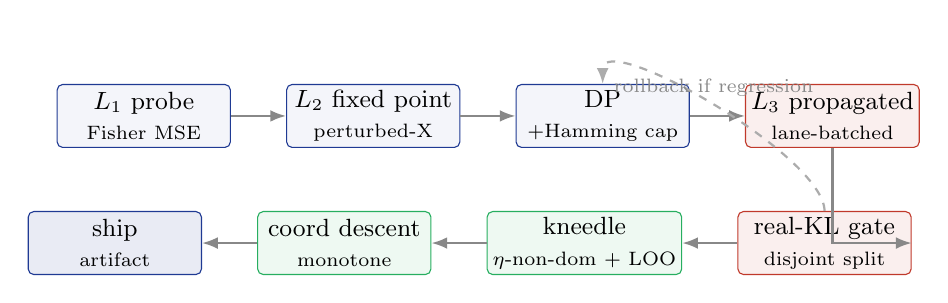
\begin{tikzpicture}[
  node distance=4mm and 7mm,
  every node/.style={font=\small},
  stage/.style={
    draw=accent, fill=accent!5, rounded corners=2pt,
    minimum height=8mm, minimum width=22mm, align=center,
    inner sep=2pt
  },
  measure/.style={
    draw=accent2, fill=accent2!8, rounded corners=2pt,
    minimum height=8mm, minimum width=22mm, align=center,
    inner sep=2pt
  },
  pick/.style={
    draw=accent3, fill=accent3!8, rounded corners=2pt,
    minimum height=8mm, minimum width=22mm, align=center,
    inner sep=2pt
  },
  arr/.style={-{Latex[length=2mm]}, thick, draw=rule}
]
  \node[stage] (probe) {$L_1$ probe\\\scriptsize Fisher MSE};
  \node[stage, right=of probe] (l2) {$L_2$ fixed point\\\scriptsize perturbed-X};
  \node[stage, right=of l2]   (dp) {DP\\\scriptsize +Hamming cap};
  \node[measure, right=of dp] (l3) {$L_3$ propagated\\\scriptsize lane-batched};
  \node[measure, below=8mm of l3, xshift=-1mm] (gate) {real-KL gate\\\scriptsize disjoint split};
  \node[pick, left=of gate]   (kneedle) {kneedle\\\scriptsize $\eta$-non-dom + LOO};
  \node[pick, left=of kneedle] (coord)   {coord descent\\\scriptsize monotone};
  \node[stage, left=of coord, fill=accent!10, draw=accent] (ship) {ship\\\scriptsize artifact};

  \draw[arr] (probe) -- (l2);
  \draw[arr] (l2)    -- (dp);
  \draw[arr] (dp)    -- (l3);
  \draw[arr] (l3.south) |- (gate.east);
  \draw[arr] (gate)  -- (kneedle);
  \draw[arr] (kneedle) -- (coord);
  \draw[arr] (coord) -- (ship);

  \draw[arr, dashed, draw=rule!70]
    (gate.north) .. controls +(0,7mm) and +(0,7mm) .. node[above, midway, font=\scriptsize, text=rule]{rollback if regression} (dp.north);
\end{tikzpicture}
\caption{The \textsc{PrismaSCOUT} pipeline. Blue stages are surrogate
candidate generation ($L_1, L_2$, additive DP). Red stages are real
measurement ($L_3$ propagated end-KL, real-KL gate on disjoint validation
split). Green stages are selection: validated-frontier kneedle and monotone
coord-descent polish. Surrogate proposals are rolled back if the real-KL gate
detects a regression.}
\label{fig:pipeline}
\end{figure}


\subsection{$L_3$ neighborhood selection}\label{subsec:l3_selection}

The $L_3$ measurement budget is bounded; we cannot afford to measure
every (Linear, format) pair on a large model. The pipeline therefore
selects a bounded \emph{neighborhood} of candidate Linears around the
converged $L_2$ assignment, prioritized as follows:
\begin{enumerate}[leftmargin=*,itemsep=1pt]
  \item \textbf{Uncertain DP choices.} Linears whose $L_2$
    second-best format is within \texttt{l3-uncertainty-rel-tol}
    (default $0.10$) of the chosen format under $u^{(2)}$. These are
    the Linears the additive DP could plausibly have flipped under a
    small perturbation of the cost.
  \item \textbf{Non-cheapest current picks.} Linears whose current
    $L_2$ choice is more expensive (in bits) than the cheapest measured
    format that does not break the bit budget elsewhere; these are the
    candidates for trading bits down with end-KL gating.
  \item \textbf{High-cost safety set.} A small fraction
    (\texttt{l3-safety-fraction}, default $0.02$) of the
    highest-predicted-cost Linears, regardless of uncertainty, to
    catch high-impact picks that were not flagged by the uncertainty
    filter.
  \item \textbf{Fill to minimum coverage.} If the above sets jointly
    cover fewer than \texttt{l3-min-fraction} (default $0.05$) of
    Linears, additional non-cheapest picks are added to reach that
    floor; the union is hard-capped at \texttt{l3-max-fraction}
    (default $0.30$).
\end{enumerate}
For each selected Linear, $L_3$ measures the current $L_2$ pick, one
cheaper format, one more accurate format, and BF16 when available; the
final DP runs only over candidates with measured $L_3$ costs and a
measured current-format candidate.

\begin{algorithm}[h]
\caption{\textsc{PrismaSCOUT} (validated-frontier knee mode)}\label{alg:scout}
\begin{algorithmic}[1]
\Require source weights $\theta$, calibration splits $C_{\mathrm{train}}$,
  $C_{\mathrm{val}}$, format menu $\Formats_i$ per Linear, anchor
  budget set $\{B_j\}$, KL noise floor $\eta$, bisection tolerance
  $\tau$
\State $u^{(1)} \gets \textsc{Probe}(\theta, C_{\mathrm{train}})$ \Comment{$L_1$ Fisher-trace probe}
\For{each anchor budget $B_j$}
  \State $\Assignment^{(0)} \gets \textsc{DP}(u^{(1)}, B_j)$
  \For{$k = 0, 1, \dots$}\Comment{$L_2$ perturbed-X fixed point}
    \State $X^{(k)} \gets \textsc{ActCache}(\theta, \Assignment^{(k)}, C_{\mathrm{train}})$
    \State $u^{(2)} \gets \textsc{MeasureLocalMSE}(\theta, X^{(k)}, \Formats)$
    \State $\Assignment^{(k+1)} \gets \textsc{DP}_{\mathrm{Hamming-cap}}(u^{(2)}, B_j, \Assignment^{(k)})$
    \If{$h^{(k)} < \texttt{convergence-frac}$} \textbf{break} \EndIf
  \EndFor
  \State $\mathcal{N} \gets \textsc{L3Neighborhood}(\Assignment^{(k)}, u^{(2)})$
  \State $u^{(3)} \gets \textsc{MeasurePropagatedKL}(\theta, \Assignment^{(k)}, \mathcal{N}, C_{\mathrm{train}})$
  \State $\Assignment_j \gets \textsc{DP}_{\mathrm{frozen}}(u^{(3)}, B_j, \mathcal{N}, \Assignment^{(k)})$
  \State $\kappa_j \gets \kl(\Assignment_j;\,C_{\mathrm{val}})$ \Comment{real-KL gate}
  \If{$\kappa_j > \kl(\Assignment^{(k)}) + \rho\,\kl(\Assignment^{(k)})$}
    $\Assignment_j \gets \Assignment^{(k)}$ \Comment{rollback}
  \EndIf
\EndFor
\State $\mathcal{F} \gets \textsc{Pareto}_{\eta}\{(\bpp(\Assignment_j),\,\kappa_j)\}$ \Comment{$\eta$-non-dominated}
\State $\Assignment^\star \gets \textsc{Kneedle}(\mathcal{F};\,\tau)$ \Comment{Equation~\eqref{eq:kneedle}}
\State $\Assignment^\star \gets \textsc{LeaveOneOutGuard}(\mathcal{F},\Assignment^\star)$
\State $\Assignment^\star \gets \textsc{CoordDescent}(\Assignment^\star,\,C_{\mathrm{val}})$ \Comment{Proposition~\ref{prop:monotone}}
\State \Return $\Assignment^\star$
\end{algorithmic}
\end{algorithm}

\subsection{The DP and fused-sibling constraints}

The allocator solves an additive multi-choice knapsack DP whose
\emph{units} are not individual Linears but \emph{refinement units} that group
fused siblings. Attention $q,k,v$ projections share a per-tensor global scale
in vLLM's fused kernel \cite{vllm}; in MoE, $\mathrm{gate\_up}$ and
$\mathrm{down}$ packed Linears must share schemes within an expert column.
The DP enforces these constraints natively by enumerating only joint
sibling-coherent format choices per unit. Fused-sibling aggregation uses
sum (joint-cost) for activation-coupled siblings and max for
isolated-sensitivity siblings; we report the rationale and an empirical
comparison in Appendix~\ref{app:fused}.

\subsection{Calibration disjointness}\label{subsec:disjoint}

The split discipline is summarized in Figure~\ref{fig:calib_split}.
\textsc{PrismaSCOUT} maintains two disjoint calibration splits:

\begin{itemize}[leftmargin=*,itemsep=2pt]
  \item \textbf{Train split} (\texttt{l3\_calib\_split=train}, default).
    Used for $L_2$ activation caching and $L_3$ paired-baseline measurement.
  \item \textbf{Validation split} (\texttt{kl\_calib\_split=validation},
    default). Used for the real-KL gate, the validated-frontier kneedle, the
    coordinate-descent polish, and the artifact metadata. Never seen by any
    cost-generation stage.
\end{itemize}

The renaming and split discipline was added in commit \texttt{2e670b3}
(``Implement PR-Polish-1: Rename validation\_kl and secure surrogate
knee'') after an audit identified that the original
\texttt{validation\_kl} field was, in fact, an in-sample number on the same
calibration split that drove $L_2$/$L_3$ cost generation. Until that fix
landed, \texttt{validation\_kl} could be reasonably misread as a held-out
metric; it was not.

\begin{figure}[t]
\centering
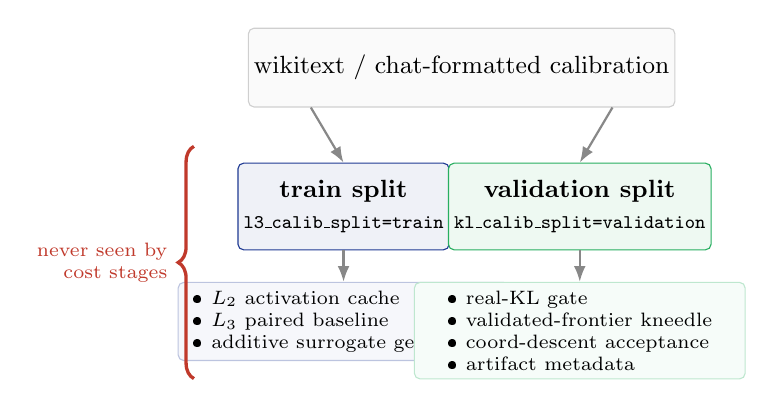
\begin{tikzpicture}[
  every node/.style={font=\small},
  block/.style={draw=accent, fill=accent!7, rounded corners=2pt,
                minimum width=24mm, minimum height=11mm, align=center, inner sep=2pt},
  block2/.style={draw=accent3, fill=accent3!8, rounded corners=2pt,
                minimum width=24mm, minimum height=11mm, align=center, inner sep=2pt},
  arr/.style={-{Latex[length=2mm]}, thick, draw=rule}
]
  \node[draw=rule!40, fill=rule!4, rounded corners=2pt,
        minimum width=46mm, minimum height=10mm, align=center, inner sep=2pt] (corpus)
    {wikitext / chat-formatted calibration};

  \node[block, below=7mm of corpus, xshift=-15mm] (train) {\textbf{train split}\\\scriptsize\texttt{l3\_calib\_split=train}};
  \node[block2, below=7mm of corpus, xshift=15mm] (val)   {\textbf{validation split}\\\scriptsize\texttt{kl\_calib\_split=validation}};

  \draw[arr] (corpus.south west) ++(8mm,0) -- (train.north);
  \draw[arr] (corpus.south east) ++(-8mm,0) -- (val.north);

  \node[draw=accent!30, fill=accent!4, rounded corners=2pt, align=left,
        below=4mm of train, inner sep=3pt, font=\scriptsize, minimum width=42mm]
    (trainuse) {\textbullet{} $L_2$ activation cache\\\textbullet{} $L_3$ paired baseline\\\textbullet{} additive surrogate generation};

  \node[draw=accent3!30, fill=accent3!4, rounded corners=2pt, align=left,
        below=4mm of val, inner sep=3pt, font=\scriptsize, minimum width=42mm]
    (valuse) {\textbullet{} real-KL gate\\\textbullet{} validated-frontier kneedle\\\textbullet{} coord-descent acceptance\\\textbullet{} artifact metadata};

  \draw[arr] (train) -- (trainuse);
  \draw[arr] (val)   -- (valuse);

  \draw[draw=accent2, very thick, decorate, decoration={brace, amplitude=2mm}]
    (-3.4, -3.95) -- (-3.4, -1.0)
    node[midway, left=2mm, font=\scriptsize, text=accent2, align=right]{never seen by\\cost stages};

\end{tikzpicture}
\caption{Calibration split discipline. The train split feeds all surrogate
cost-generation stages ($L_2$ activation cache, $L_3$ paired baseline,
additive DP). The validation split feeds every selection decision
(real-KL gate, kneedle, coord descent, artifact metadata) and is never
seen by any cost stage. Until commit \texttt{2e670b3} (PR-Polish-1), the
field labelled \texttt{validation\_kl} could be reasonably misread as
held-out; that field has been renamed throughout to require disjoint splits
in the shipping path.}
\label{fig:calib_split}
\end{figure}


\section{Methods Considered and Rejected}\label{sec:rejected}

The shipping algorithm above is the result of a deliberate triangulation
between several principled alternatives. We describe each, the math behind
it, and the empirical or structural reason it was not adopted as the default.
The intent is not exhaustiveness for its own sake --- it is to make explicit
that simpler, mathematically attractive answers were considered first.
Figure~\ref{fig:methods_tree} catalogs the full set, classified as
shipped, experimental, or rejected.

\subsection{Lagrangian \texorpdfstring{$\lambda$}{lambda}-bisection on the dual gradient}\label{subsec:lambda}

\paragraph{The proposal.} The constrained problem
$\min_\Assignment U(\Assignment)\;\text{s.t.}\;B(\Assignment) \le B$ admits the
Lagrangian relaxation $L(\Assignment, \lambda) = U(\Assignment) + \lambda(B(\Assignment) - B)$.
Sweeping $\lambda$ traces the lower convex envelope of the achievable
$(\bpp,\,U)$ frontier. For each $\lambda$, the per-Linear minimizer
decouples: $\Assignment_i^\star(\lambda) = \arg\min_f\,u_i(f) + \lambda\,
b_i(f)$ where $b_i(f)$ is the bit count for Linear $i$ at format $f$. This
costs CPU seconds. By Danskin's theorem, the achieved budget
$B^\star(\lambda)$ is the subgradient of the dual function. The kneedle is
the region of maximum $|dB^\star/d\lambda|$ on log-$\lambda$. A few-step
bisection on $\lambda$ produces the kneedle without sweeping the full grid.

\paragraph{Theoretical optimality.} For a strictly convex frontier, the
proposal is optimal: $5$--$7$ $\lambda$ evaluations isolate the kneedle
to within $0.04$ bpp.

\paragraph{Why we did not adopt it as the default.} Two reasons.

First, the discrete frontier is not strictly convex. Sub-bit combinatorial
packing produces concave pockets where a slightly suboptimal assignment lies
\emph{above} the convex hull. No strictly positive $\lambda$ selects those
points as global minimizers of $L$; sweeping $\lambda$ leaps over them. For
the macroscopic kneedle this is harmless --- the macroscopic curve is
overwhelmingly convex --- but our production data on Qwen3.6-27B exhibits a
non-trivial gap between the surrogate-only knee at 5.857~bpp / measured
KL~0.056 and the validated-frontier knee at 5.31~bpp / measured KL~0.015
(Figure~\ref{fig:lambda_skip}). The validated-frontier kneedle and the
discrete archive-DP candidate set both find the 5.31 point; a pure
$\lambda$-sweep on the surrogate does not.

Second, the surrogate $U_{\mathrm{add}}$ used inside the Lagrangian is the
same additive quantity whose joint behavior overshoots true KL by 30--50\%.
Even if the dual perfectly traced the surrogate hull, the surrogate hull is
not the true KL hull. We therefore retained a \emph{$\lambda$-archive search}
as an experimental candidate generator (commit \texttt{86f2c14}, ``Add
lambda archive knee search''; commit \texttt{444bc28}, ``Add one-pass Pareto
archive DP''), with a beam variant retaining alternate states per bit bin.
But the final selector is real-KL on the validated frontier; the
$\lambda$-archive feeds candidates into that selector, not the other way
around.

\begin{figure}[t]
\centering
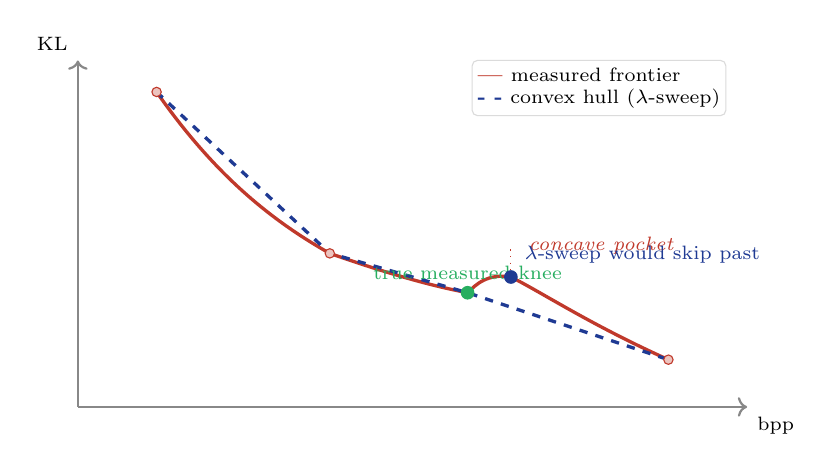
\begin{tikzpicture}[
  every node/.style={font=\small},
  axis/.style={->, thick, draw=rule}
]
  \def\xa{0}\def\xb{8.5}\def\ya{0}\def\yb{4.4}
  \draw[axis] (\xa,\ya) -- (\xb,\ya) node[below right, font=\scriptsize]{$\bpp$};
  \draw[axis] (\xa,\ya) -- (\xa,\yb) node[above left, font=\scriptsize]{KL};

  % "True" measured frontier with concave segment
  \draw[draw=accent2, very thick]
    (1.0, 4.0) .. controls (1.7, 3.0) and (2.4, 2.4) ..
    (3.2, 1.95)
    .. controls (4.2, 1.6) and (4.7, 1.5) ..
    (4.95, 1.45)               % concave segment up
    .. controls (5.05, 1.55) and (5.2, 1.7) ..
    (5.5, 1.65)                % bump up
    .. controls (5.9, 1.45) and (6.5, 1.05) ..
    (7.5, 0.6);

  % Convex hull (skips the bump)
  \draw[draw=accent, very thick, dashed]
    (1.0, 4.0) -- (3.2, 1.95) -- (4.95, 1.45) -- (7.5, 0.6);

  % Frontier points
  \foreach \x/\y in {1.0/4.0, 3.2/1.95, 4.95/1.45, 5.5/1.65, 7.5/0.6} {
    \node[circle, draw=accent2, fill=accent2!30, inner sep=1.2pt] at (\x, \y) {};
  }

  % Concave-skip annotation
  \node[font=\scriptsize, anchor=west, text=accent2] at (5.6, 2.05)
    {\itshape concave pocket};
  \draw[draw=accent2, dotted] (5.5, 2.0) -- (5.5, 1.7);

  % Knee labels
  \node[circle, draw=accent3, fill=accent3, inner sep=1.6pt] (truek) at (4.95, 1.45) {};
  \node[font=\scriptsize, text=accent3, anchor=south] at (4.95, 1.5) {true measured knee};

  \node[circle, draw=accent, fill=accent, inner sep=1.6pt] (lamk) at (5.5, 1.65) {};
  \node[font=\scriptsize, text=accent, anchor=south west] at (5.55, 1.7) {$\lambda$-sweep would skip past};

  % Legend
  \node[font=\scriptsize, anchor=west, draw=rule!30, fill=white, rounded corners=2pt, inner sep=2pt]
    at (5.0, 4.05)
    {\begin{tabular}{@{}l@{}}
      {\color{accent2}\textbf{---}} measured frontier\\
      {\color{accent}\textbf{- -}} convex hull ($\lambda$-sweep)
    \end{tabular}};
\end{tikzpicture}
\caption{Why a Lagrangian $\lambda$-sweep is not the shipping selector.
The achievable mixed-precision frontier (red) admits non-convex
``pockets'' --- combinatorially-suboptimal assignments that lie
\emph{above} the lower convex hull. A $\lambda$-sweep traces the dashed
hull and never selects pocket points; for the macroscopic kneedle this is
harmless, but on the Qwen3.6-27B production data the gap between the
hull-knee at $5.857$\,bpp and the measured-frontier knee at $5.31$\,bpp
is operationally meaningful. We retain the $\lambda$-archive search as a
candidate generator and gate selection on real KL.}
\label{fig:lambda_skip}
\end{figure}


\subsection{Sandwich proximal recalibration}

\paragraph{The proposal.} The non-additivity bug is a Taylor-trust-region
bug: $u^{(2)}_i$ is measured holding $\Assignment_{-i}$ at $\Assignment^{(\mathrm{ref})}$,
the DP then proposes a multi-flip $\Assignment^{(\mathrm{prop})}$ far outside
that radius. The remedy proposed in the design deliberation
\cite[\texttt{scratch/deliberation/02\_gemini.md}]{prismaquant} is a
\emph{sandwich}: propose $\Assignment^{(\mathrm{prop})}$ from the additive
DP, re-measure $u^{(2)}_i$ holding $\Assignment_{-i}$ at
$\Assignment^{(\mathrm{prop})}$, re-solve the DP. Under a Mirror-Descent
analysis with contraction factor $\rho$ equal to the ratio of off-diagonal
to block-diagonal Hessian energy --- which the deliberation estimated at
$\rho \in [0.3, 0.5]$ from the observed $\mathrm{KL}_{\mathrm{prop}} /
\mathrm{KL}_{\mathrm{DP}} \in [1.3, 1.5]$ overshoot ratio --- $2$--$3$
sandwich passes are predicted to reach within $5\%$ of the true KL
minimum. We did not run the sandwich loop end-to-end, so this estimate is
analytic, not empirical.

\paragraph{Why not adopted as default.} Two practical reasons.

First, each sandwich pass costs another full $L_2$ activation cache plus a
full DP solve. On Qwen3.6-27B, each pass is $\sim$22 minutes wall, so 3
passes is over an hour per anchor. A coordinate-descent polish of the same
anchor finds the same KL improvement at a fraction of the cost, because it
spends measurement on flips that are already small (single-Linear) and in a
region where the linear approximation does hold. Coord descent is also
trivially monotone on real KL by construction, while sandwich is
\emph{empirically} contractive.

Second, the operational re-centering target is the \emph{actual} chosen
assignment, not a sequence of $L_2$ DP outputs. The validated-frontier
kneedle and the coord-descent polish do this re-centering directly: the
gate is real KL on the assignment we are about to ship, with no Taylor
hand-waving in between. Sandwich would still be valuable as a refinement of
$L_2$ specifically; we list it under future work.

\subsection{Block-DP over architectural cliques}

\paragraph{The proposal.} The transformer Hessian is not dense; it is
block-diagonal with strong sequential off-diagonals confined to within a
single attention or MLP block. The structurally non-zero pairwise
interactions are essentially:

\[
  \mathrm{V}_{\mathrm{proj}} \to \mathrm{O}_{\mathrm{proj}}, \qquad
  \mathrm{Gate}_{\mathrm{proj}}/\mathrm{Up}_{\mathrm{proj}} \to \mathrm{Down}_{\mathrm{proj}}.
\]

A block-DP over these cliques (size $2$--$3$, disjoint after LayerNorm
resets, illustrated in Figure~\ref{fig:smrf_clique}) captures the dominant
interaction energy without an NP-hard QUBO, in
$K = 2 \cdot \mathrm{num\_layers}$ measurements per pass.

\begin{figure}[t]
\centering
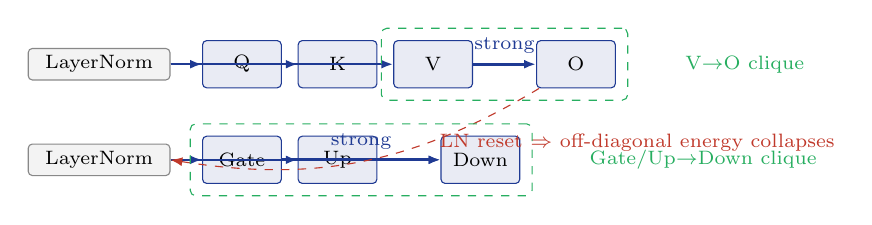
\begin{tikzpicture}[
  every node/.style={font=\scriptsize},
  proj/.style={
    draw=accent, fill=accent!10, rounded corners=1.5pt,
    minimum height=6mm, minimum width=10mm, inner sep=1pt
  },
  norm/.style={
    draw=rule, fill=rule!10, rounded corners=1.5pt,
    minimum height=4mm, minimum width=18mm, inner sep=1pt
  },
  edge/.style={-{Latex[length=1.5mm]}, draw=accent, thick},
  longedge/.style={-{Latex[length=1.5mm]}, dashed, draw=accent2}
]
  % Block 1: attention
  \node[norm] (ln1) at (0,0) {LayerNorm};
  \node[proj, right=4mm of ln1] (q) {Q};
  \node[proj, right=2mm of q]   (k) {K};
  \node[proj, right=2mm of k]   (v) {V};
  \node[proj, right=8mm of v]   (o) {O};

  \draw[edge] (ln1) -- (q.west);
  \draw[edge] (ln1) -- (k.west);
  \draw[edge] (ln1) -- (v.west);
  \draw[edge, very thick] (v) -- (o)
    node[midway, above, font=\scriptsize, text=accent]{strong};

  % MLP block
  \node[norm, below=8mm of ln1] (ln2) {LayerNorm};
  \node[proj, right=4mm of ln2] (gate) {Gate};
  \node[proj, right=2mm of gate] (up)  {Up};
  \node[proj, right=8mm of up]   (down) {Down};

  \draw[edge] (ln2) -- (gate.west);
  \draw[edge] (ln2) -- (up.west);
  \draw[edge, very thick] (gate) -- (down)
    node[midway, above, font=\scriptsize, text=accent]{strong};
  \draw[edge, very thick] (up) -- (down);

  % Cross-block edges (rejected by LN reset)
  \draw[longedge] (o) to[bend left=20] (ln2.east);
  \node[font=\scriptsize, text=accent2, anchor=west] at (4.2, -1.0)
    {LN reset $\Rightarrow$ off-diagonal energy collapses};

  % Annotation: cliques
  \node[draw=accent3, dashed, rounded corners=2pt, fit=(v)(o), inner sep=1.5mm] (att_clique) {};
  \node[draw=accent3, dashed, rounded corners=2pt, fit=(gate)(up)(down), inner sep=1.5mm] (mlp_clique) {};
  \node[font=\scriptsize, text=accent3, anchor=west] at ($(att_clique.east)+(0.6,0)$) {V$\to$O clique};
  \node[font=\scriptsize, text=accent3, anchor=west] at ($(mlp_clique.east)+(0.6,0)$) {Gate/Up$\to$Down clique};

\end{tikzpicture}
\caption{Architectural cliques in transformer blocks. The dominant
non-additive interactions in mixed-precision quantization are confined to
the V$\to$O attention output projection and the Gate/Up$\to$Down MLP
output projection. LayerNorms reset error magnitude between blocks, so
cross-block off-diagonal Hessian energy is small. A block-DP over these
disjoint cliques (Section~\ref{sec:rejected}) would in principle capture
the structural interaction without an NP-hard QUBO. We do not adopt it as
a default because the additive DP's fused-sibling refinement units already
absorb the within-clique constraint via joint sibling-coherent format
choices.}
\label{fig:smrf_clique}
\end{figure}


\paragraph{Why not adopted as default.} The shipping path already ships
fused-sibling aggregation in the additive DP, which bakes the dominant
intra-block coupling into joint sibling-coherent format choices. The
$\mathrm{Gate}/\mathrm{Up}\to\mathrm{Down}$ correlation is already
treated jointly inside the refinement unit. Block-DP would extend this to
$\mathrm{V}\to\mathrm{O}$, which is real, but not large enough on the
configurations we measured to justify a measurement pass beyond the existing
sibling aggregation. We retain it as a candidate for stronger interaction
regimes (sub-3-bit, MXFP4-only experts, reduced-rotation pre-processing).

\subsection{Sparse pairwise QUBO / SMRF}

\paragraph{The proposal.} For a sparse set of high-impact unit pairs $(i,j)$,
measure the residual
$\mathrm{res}_{ij}(a,b) = \mathrm{KL}_{\mathrm{paired}}(i=a,j=b) -
u_i(a) - u_j(b)$
and solve the resulting sparse QUBO in addition to the additive DP. This is
implemented in \texttt{interaction\_refine.py}.

\paragraph{Why default-off.} On the production Qwen3.6-27B run, the pairwise
stage covered 8 high-impact units at the cost of $\sim$250 paired forwards
($\sim$45 minutes) and rolled back when validation regressed. Coverage of
8 units out of $\sim$500 Linears is what one of our reviewers (Gemini~3.1)
called \emph{homeopathic}: too local to fix global non-additivity and
expensive enough to dominate the budget when activated. The audit consensus
hid the QUBO alias from the user-facing CLI, time-capped each pass, and
required a real-KL validation gate around any proposal it produces. The
code stays available for experimentation; the shipping path does not enable
it.

\subsection{Top-\texorpdfstring{$K$}{K} Hessian-eigenvalue covering}

\paragraph{The proposal.} Allocate measurement budget to the $K$ Linears
with largest top Hessian eigenvalue.

\paragraph{Why rejected.} The eigenvalue ranks individual matrices by local
sensitivity. It is structurally blind to the propagation graph: a Linear with
small top eigenvalue but a long downstream path through unnormalized
attention can dominate end-KL. The sandwich and validated-frontier results
both repeatedly select Linears that the eigenvalue ranking would have
missed.

\subsection{Surrogate-only knee selection}\label{subsec:surrogate}

\paragraph{The proposal.} Sweep target $\bpp$ on a single cached $L_3$ cost
table; let $U_{\mathrm{add}} = \sum_i u^{(3)}_i(\Assignment_i)$ stand in for
KL; pick the kneedle on the surrogate frontier.

\paragraph{Why rejected.} On the Qwen3.6-27B production data
(Figure~\ref{fig:validated_27b}), the surrogate kneedle picks
5.857~bpp / KL~0.056. The validated kneedle on the same candidate set picks
5.31~bpp / KL~0.015. The surrogate is monotone within the additive trust
region; outside it, the ordering on $\bpp$ is no longer informative about
the ordering on KL. We retain the surrogate sweep as an
extremely cheap candidate generator (CPU seconds for hundreds of points)
and pair it with an obligatory \texttt{--knee-surrogate-validate} gate that
re-measures the picked points on real KL. After PR-Polish-1, the
surrogate-only path is hidden from the user-facing CLI; outputs are
relabeled \texttt{candidate\_surrogate\_*} so a reader cannot mistake the
surrogate kneedle for the shipping artifact.

\subsection{Probe-only knee prediction}

\paragraph{The proposal.} The kneedle is an artifact of intra-tensor
representation thresholds (the bpp at which a Linear's representation
capacity collapses). The $L_1$ probe captures those thresholds well. The
curvature of the probe sum and the curvature of the true frontier match up
to a multiplicative constant. Predict the knee bpp from $L_1$ alone.

\paragraph{Why used as a prior, not a selector.} On Qwen-4B-class scales the
expected error in the probe-predicted knee is empirically $\pm 0.12$--$0.18$
bpp \cite{prismaquant}. The density of mixed-precision states near the true
knee is often $\le 0.05$ bpp. A $\pm 0.15$ bpp error therefore guarantees we
miss the exact discrete kneedle. The probe is the optimal prior for
\emph{bracket} establishment (e.g., search in $[3.8, 4.1]$ bpp), but the
final discrete selection requires a real-KL evaluation of $3$--$5$
$\lambda$- or DP-generated candidates within that bracket.

\subsection{Pareto archive DP and beam variants}

\paragraph{The proposal.} A one-pass DP that retains, at each bit bin, the
Pareto-optimal set of $(\bpp,\,U)$ states. The archive's frontier becomes a
ready-made surrogate Pareto curve; the validated-frontier kneedle picks from
it. The beam variant
(\texttt{-{}-knee-archive-beam-per-bin}) retains $k$ alternate states per
bin. The refinement stage adds neighbors of the current best measured KL.

\paragraph{Status.} Implemented and flag-gated as candidate generation
(commit \texttt{444bc28} for one-pass DP, beam variant in commit
\texttt{53fe0db}). The archive feeds candidates into the validated-frontier
selector when enabled via \texttt{-{}-knee-archive-*} flags; it does not
replace the validated-frontier kneedle as the final selector. The
production Qwen3.6-27B archive run
(\texttt{27b-knee-archive-beam4-refine-noseed}) is the canonical example:
its no-seed selection was $5.31$~bpp / measured KL $0.0147$, about $9.9\%$
relative KL worse than a separately-supplied best assignment at
$5.27$~bpp / KL $0.0134$. We treat archive DP as a high-coverage candidate
generator, audited by the same real-KL gate as the rest of the pipeline.

\subsection{Top-down (ceiling-start) production-faithful polish}\label{subsec:topdown}

\paragraph{The proposal.} Mirror the bottom-up production-faithful polish
(Section~\ref{subsec:prodpolish}) by starting at the all-BF16 ceiling and
accepting flips that strictly decrease total bits while keeping real KL
within a small budget. Two trajectories from opposite endpoints ought to
sandwich the achievable Pareto interior, and their union ought to give
much denser frontier coverage than either alone --- a symmetric two-trajectory
sandwich.

\paragraph{Why default-off.} On Qwen3.6-27B, the bottom-up forward pass
committed $12$ accepted moves in $1706$~s and reached the
$5\%$ bits-budget creep. The top-down pass with the symmetric
\texttt{max\_passes}=$12$ cap committed $12$ accepted moves in $13$~s ---
two orders of magnitude faster wall-time per accept --- and consumed only
$0.05\%$ of its KL budget ($0.0023$ of an allowed $0.05$). The two
trajectories did not overlap: forward stayed near $5.39$~bpp, top-down
stayed near $15.62$~bpp, and the entire interior was empty. The cause is
the move set's geometry: starting from all-BF16, every candidate flip is
a $\sim 12$-bit reduction (BF16 $\to$ NVFP4) at near-zero KL cost, so the
greedy chooses the unit with the smallest KL increase among those, finds
many nearly-identical such picks at the start, and uses the entire
\texttt{max\_passes} budget on cheap flips with no incentive to
extend toward the bpp range where the forward sweep operates. Increasing
\texttt{max\_passes} to $100$+ would in principle close the gap by
exhausting the KL budget --- the contractual stopping condition for the
top-down direction is that no further bits-decreasing flip stays under
$\kappa_{\mathrm{budget}}$, which on Qwen3.6-27B at
$\kappa_{\mathrm{budget}} = 0.05$ means many more accepted flips than
\texttt{max\_passes}=12 allowed. But the top-down direction also has no
convergence guarantee \emph{toward a knee}: it descends until the KL
budget is the binding constraint, which is operationally equivalent to
``find the highest-bpp assignment with KL just under the budget'', not
``find the right Pareto-optimal point''. We retired the top-down
direction; the shipping production-faithful polish runs only the
bottom-up sweep from the floor.

\paragraph{What we kept from the experiment.} The plumbing
(\texttt{--direction top\_down}, \texttt{--kl-budget}) stays in
\texttt{polish\_from\_assignment} for symmetric experimentation, gated off
by default. The defensive
\texttt{member\_qnames}-coverage assertion in
\texttt{coord\_descent\_polish} that this round added is unconditional ---
both directions would have silently produced wrong bits accounting under
the original payload-key bug.

\subsection{The UMA-clone misadventure}\label{subsec:umaclone}

\paragraph{The proposal.} On a 121~GB UMA host, polish on a 27B model
runs out of memory if every trial clones the candidate Linear's weight in
GPU-resident memory. A natural-looking remedy is to clone the slot to
\emph{CPU} between trials and copy back on demand: CPU memory and GPU
memory are different pools, so the trial-time peak should drop.

\paragraph{Why structurally wrong.} The GB10 is a unified-memory device:
the CPU and GPU share the same physical pool. ``Move to CPU'' relabels a
tensor as host-resident in the PyTorch view but does not change which
DRAM page backs it; the trial-time peak is identical. The right fix is
not to clone the \emph{whole materialized model} per trial: the
\texttt{WeightSession} delta-quantize path
(Section~\ref{subsec:prodpolish}) still clones the staged unit's slot
on each trial (so a revert is a $\sim$50--500~MB \texttt{copy\_} per
unit, not free), but it eliminates the $\sim$54~GB-per-trial full-model
clone that the per-module hook path used to make. We mention the
non-fix because it is a recurring class of mistake on UMA architectures:
a memory-management heuristic that is correct on a discrete-GPU host can
be a no-op on a UMA host, and the eviction path of the
\texttt{ProductionWeightCache}'s LRU was designed against a discrete-GPU
mental model before being re-derived under the UMA assumption. The
production cache now disk-streams (one \texttt{.pt} per (qname, fmt)
pair) rather than relying on host/device pool separation, with an
LRU bound on resident-tensor bytes.

\begin{figure}[t]
\centering
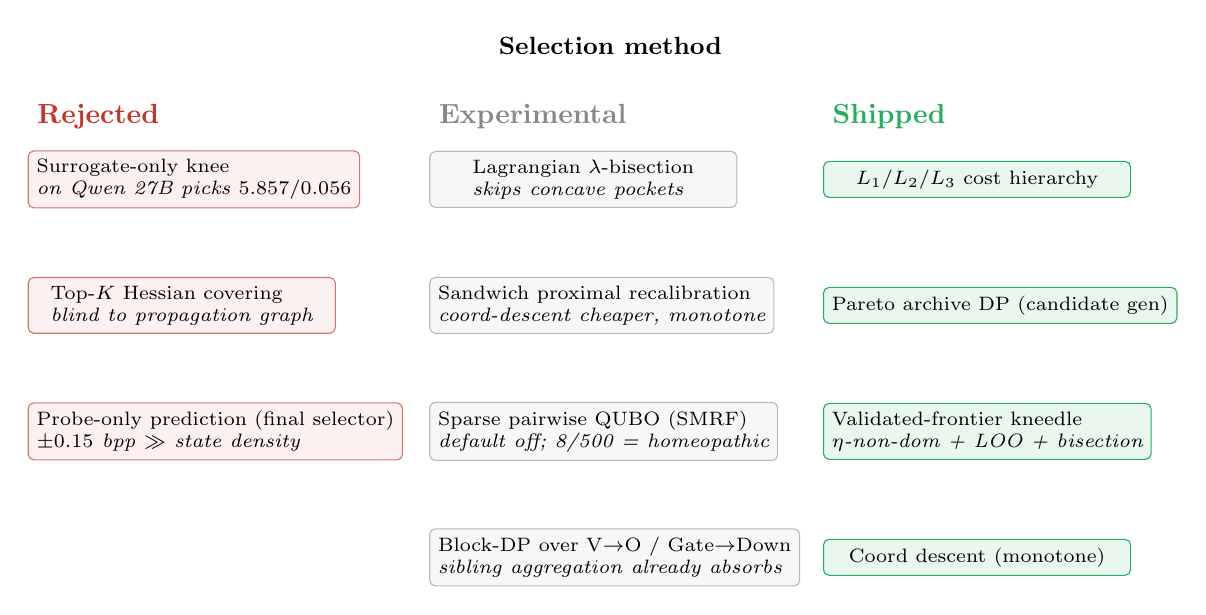
\begin{tikzpicture}[
  every node/.style={font=\scriptsize},
  rejected/.style={draw=accent2!70, fill=accent2!7, rounded corners=2pt,
                   align=left, inner sep=3pt, minimum width=39mm},
  experimental/.style={draw=rule!60, fill=rule!7, rounded corners=2pt,
                       align=left, inner sep=3pt, minimum width=39mm},
  shipped/.style={draw=accent3, fill=accent3!10, rounded corners=2pt,
                  align=left, inner sep=3pt, minimum width=39mm},
  arr/.style={-{Latex[length=1.6mm]}, draw=rule}
]
  \node[font=\small\bfseries] (root) at (0, 0) {Selection method};

  % Three columns: rejected, experimental, shipped
  \node[font=\bfseries, text=accent2,  anchor=west] at (-7.4, -0.9) {Rejected};
  \node[font=\bfseries, text=rule,     anchor=west] at (-2.3, -0.9) {Experimental};
  \node[font=\bfseries, text=accent3,  anchor=west] at ( 2.7, -0.9) {Shipped};

  % Rejected
  \node[rejected, anchor=west] (r1) at (-7.4, -1.7)
    {Surrogate-only knee\\\itshape on Qwen 27B picks $5.857/0.056$};
  \node[rejected, anchor=west] (r2) at (-7.4, -3.3)
    {Top-$K$ Hessian covering\\\itshape blind to propagation graph};
  \node[rejected, anchor=west] (r3) at (-7.4, -4.9)
    {Probe-only prediction (final selector)\\\itshape $\pm 0.15$ bpp $\gg$ state density};

  % Experimental
  \node[experimental, anchor=west] (e1) at (-2.3, -1.7)
    {Lagrangian $\lambda$-bisection\\\itshape skips concave pockets};
  \node[experimental, anchor=west] (e2) at (-2.3, -3.3)
    {Sandwich proximal recalibration\\\itshape coord-descent cheaper, monotone};
  \node[experimental, anchor=west] (e3) at (-2.3, -4.9)
    {Sparse pairwise QUBO (SMRF)\\\itshape default off; 8/500 = homeopathic};
  \node[experimental, anchor=west] (e4) at (-2.3, -6.5)
    {Block-DP over V$\to$O / Gate$\to$Down\\\itshape sibling aggregation already absorbs};

  % Shipped
  \node[shipped, anchor=west] (s1) at (2.7, -1.7)
    {$L_1$/$L_2$/$L_3$ cost hierarchy};
  \node[shipped, anchor=west] (s2) at (2.7, -3.3)
    {Pareto archive DP (candidate gen)};
  \node[shipped, anchor=west] (s3) at (2.7, -4.9)
    {Validated-frontier kneedle\\\itshape $\eta$-non-dom + LOO + bisection};
  \node[shipped, anchor=west] (s4) at (2.7, -6.5)
    {Coord descent (monotone)};

\end{tikzpicture}
\caption{Methods considered during design, classified by status. \emph{Shipped}
(green) is the production path. \emph{Experimental} (gray) is implemented
in the codebase but disabled or hidden from the user-facing CLI; remains
available for stronger interaction regimes. \emph{Rejected} (red) was
proposed and analyzed but did not survive empirical or structural
analysis. Each method is principled in its regime; the column it lands in
reflects whether that regime matches modern transformer
mixed-precision allocation under a real-KL gate.}
\label{fig:methods_tree}
\end{figure}


\section{Engineering Considerations}\label{sec:engineering}

The theoretical framework requires real-KL measurement to dominate
selection. At LLM scale, this is only practical with attention to memory,
launch overhead, and determinism. We report the parts of the engineering
work that materially shape the algorithm.

\subsection{The 128~GB UMA constraint}

The development host is an NVIDIA GB10 (Blackwell) with 128~GB unified
memory shared between GPU and host. Quantization workloads at Qwen-27B scale
have a non-trivial peak memory schedule
(Figure~\ref{fig:memory_landscape}):
model weights $\sim$54~GB BF16, $L_2$ activation cache up to 24~GB across
iterations, frozen-weight cache $\sim$4~GB, lane-batched activations
$\sim$3$-$5~GB, CUDA graph pools $\sim$10$-$20~GB if naively stacked,
Triton kernel JIT transients $\sim$1$-$2~GB, and Python plus framework
baseline $\sim$3~GB. Single-component runs fit cleanly. All-on stacks reach
99--120~GB and OOM-kill, sometimes silently before the in-process budget
enforcer can intervene.

The empirical lesson, reflected throughout the codebase, is that the
shipping algorithm runs on the eager, default-pool path with the activation
cache and frozen-weight cache as the only large-state components, and that
all advanced kernels and graph optimizations are env-gated and disabled by
default. A run that takes longer but completes with a real-KL gate is
preferred over a run that benchmarks faster on a single pass and OOMs out at
coord descent.

\begin{figure}[t]
\centering
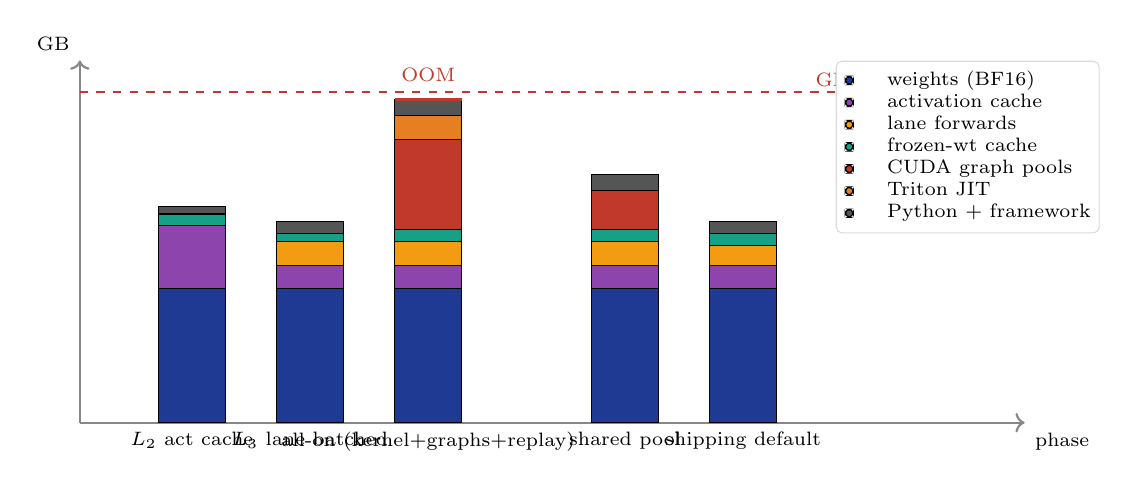
\begin{tikzpicture}[
  every node/.style={font=\small},
  axis/.style={->, thick, draw=rule}
]
  % Horizontal axis = phase, vertical axis = GB
  \def\xa{0}\def\xb{12.0}\def\ya{0}\def\yb{4.6}
  \draw[axis] (\xa,\ya) -- (\xa,\yb) node[above left, font=\scriptsize]{GB};
  \draw[axis] (\xa,\ya) -- (\xb,\ya) node[below right, font=\scriptsize]{phase};

  % UMA cap line
  \draw[draw=accent2, dashed, thick] (\xa, 4.2) -- (\xb-0.05, 4.2);
  \node[anchor=east, font=\scriptsize, text=accent2] at (\xb-0.1, 4.35) {GB10 128\,GB UMA};

  % Stacked bars: each bar is one phase, components stack
  % phase widths
  \def\bw{0.85}
  % Reusable colors
  \definecolor{cWeights}{HTML}{1f3a93}
  \definecolor{cAct}{HTML}{8e44ad}
  \definecolor{cFroz}{HTML}{16a085}
  \definecolor{cLane}{HTML}{f39c12}
  \definecolor{cGraphs}{HTML}{c0392b}
  \definecolor{cTriton}{HTML}{e67e22}
  \definecolor{cBase}{HTML}{555555}

  % Stack helper: just type out each bar
  % bar = (xc, [components])
  % L2 fixed point phase
  \draw[fill=cWeights] (1.0, 0)        rectangle (1.0+\bw, 1.7);  % weights 54GB scaled
  \draw[fill=cAct]     (1.0, 1.7)      rectangle (1.0+\bw, 2.5);  % L2 act cache
  \draw[fill=cFroz]    (1.0, 2.5)      rectangle (1.0+\bw, 2.65); % frozen wt cache
  \draw[fill=cBase]    (1.0, 2.65)     rectangle (1.0+\bw, 2.75); % base
  \node[anchor=north, font=\scriptsize] at (1.0+\bw/2, 0) {$L_2$ act cache};

  % L3 lane batched phase
  \draw[fill=cWeights] (2.5, 0)        rectangle (2.5+\bw, 1.7);
  \draw[fill=cAct]     (2.5, 1.7)      rectangle (2.5+\bw, 2.0);
  \draw[fill=cLane]    (2.5, 2.0)      rectangle (2.5+\bw, 2.3);
  \draw[fill=cFroz]    (2.5, 2.3)      rectangle (2.5+\bw, 2.4);
  \draw[fill=cBase]    (2.5, 2.4)      rectangle (2.5+\bw, 2.55);
  \node[anchor=north, font=\scriptsize] at (2.5+\bw/2, 0) {$L_3$ lane batched};

  % All-on (kernel + graphs + replay) — OOM
  \draw[fill=cWeights] (4.0, 0)        rectangle (4.0+\bw, 1.7);
  \draw[fill=cAct]     (4.0, 1.7)      rectangle (4.0+\bw, 2.0);
  \draw[fill=cLane]    (4.0, 2.0)      rectangle (4.0+\bw, 2.3);
  \draw[fill=cFroz]    (4.0, 2.3)      rectangle (4.0+\bw, 2.45);
  \draw[fill=cGraphs]  (4.0, 2.45)     rectangle (4.0+\bw, 3.6);  % CUDA graphs naive
  \draw[fill=cTriton]  (4.0, 3.6)      rectangle (4.0+\bw, 3.9);
  \draw[fill=cBase]    (4.0, 3.9)      rectangle (4.0+\bw, 4.1);
  \draw[draw=accent2, very thick] (4.0, 4.1) -- (4.0+\bw, 4.1)
    node[midway, above=1mm, font=\scriptsize, text=accent2]{OOM};
  \node[anchor=north, font=\scriptsize] at (4.0+\bw/2, 0) {all-on (kernel+graphs+replay)};

  % Shared pool config
  \draw[fill=cWeights] (6.5, 0)        rectangle (6.5+\bw, 1.7);
  \draw[fill=cAct]     (6.5, 1.7)      rectangle (6.5+\bw, 2.0);
  \draw[fill=cLane]    (6.5, 2.0)      rectangle (6.5+\bw, 2.3);
  \draw[fill=cFroz]    (6.5, 2.3)      rectangle (6.5+\bw, 2.45);
  \draw[fill=cGraphs]  (6.5, 2.45)     rectangle (6.5+\bw, 2.95);  % shared pool 1 instead of 4
  \draw[fill=cBase]    (6.5, 2.95)     rectangle (6.5+\bw, 3.15);
  \node[anchor=north, font=\scriptsize] at (6.5+\bw/2, 0) {shared pool};

  % Shipping default (eager)
  \draw[fill=cWeights] (8.0, 0)        rectangle (8.0+\bw, 1.7);
  \draw[fill=cAct]     (8.0, 1.7)      rectangle (8.0+\bw, 2.0);
  \draw[fill=cLane]    (8.0, 2.0)      rectangle (8.0+\bw, 2.25);
  \draw[fill=cFroz]    (8.0, 2.25)     rectangle (8.0+\bw, 2.4);
  \draw[fill=cBase]    (8.0, 2.4)      rectangle (8.0+\bw, 2.55);
  \node[anchor=north, font=\scriptsize] at (8.0+\bw/2, 0) {shipping default};

  % Legend
  \node[anchor=west, font=\scriptsize, draw=rule!30, fill=white, rounded corners=2pt, inner sep=3pt]
    at (9.6, 3.5)
    {\begin{tabular}{@{}cl@{}}
      \tikz \filldraw[fill=cWeights] (0,0) rectangle (3pt,3pt); & weights (BF16) \\
      \tikz \filldraw[fill=cAct] (0,0) rectangle (3pt,3pt); & activation cache \\
      \tikz \filldraw[fill=cLane] (0,0) rectangle (3pt,3pt); & lane forwards \\
      \tikz \filldraw[fill=cFroz] (0,0) rectangle (3pt,3pt); & frozen-wt cache \\
      \tikz \filldraw[fill=cGraphs] (0,0) rectangle (3pt,3pt); & CUDA graph pools \\
      \tikz \filldraw[fill=cTriton] (0,0) rectangle (3pt,3pt); & Triton JIT \\
      \tikz \filldraw[fill=cBase] (0,0) rectangle (3pt,3pt); & Python + framework
    \end{tabular}};
\end{tikzpicture}
\caption{Memory landscape on the GB10 development host (Qwen3.6-27B
configuration; bar heights illustrative, drawn to relative scale).
Single-component runs fit cleanly. The naive ``all-on'' configuration
(per-path CUDA graph pools + Triton-fused NVFP4 kernel + replay cache)
stacks past the 128\,GB UMA cap and OOM-kills. The shared-pool
configuration consolidates four graph pools into one workspace and recovers
$\sim$10\,GB. The shipping default eager-pool path with bounded LRU caches
is the rightmost bar; it is what produces the published artifacts.}
\label{fig:memory_landscape}
\end{figure}


\subsection{Lane-batched $L_3$ measurement}

The $L_3$ measurement of one (Linear, format) candidate forwards a calibration
batch through the model with one Linear in BF16 and one Linear at the
candidate format. Naively, each candidate is a separate forward. Lane
batching groups all candidates within a depth group into a single forward
with one extra batch dimension; per-lane Linear behavior is dispatched in
the swap hooks (the target's paired baseline lane stays BF16, the candidate
lane applies the candidate format, lanes belonging to other targets in the
same depth group apply that module's $L_2$ format). This reduced launch
overhead by 30$-$60$\times$ versus the sequential implementation, at the
cost of activation memory linear in the number of lanes; the
\texttt{-{}-l3-max-lanes-per-batch} flag bounds memory.

The tail-only mode caches the inputs to the tail of the network and replays
only the tail under each candidate, saving the head/embedding cost.
\texttt{PRISMAQUANT\_L3\_MIN\_HOST\_MEM\_GB} adds memory backpressure for
UMA hosts: the loop checks \texttt{/proc/meminfo} \texttt{MemAvailable}
between paired-override chunks and reduces the next chunk's lane count
before the host reaches OOM pressure.

\subsection{CUDA graphs and the shared-pool retreat}

CUDA graph capture eliminates per-launch overhead for the fixed-shape forward
paths used in $L_2$, $L_3$, KL evaluation, and coordinate-descent flip
evaluation. Naive capture allocates a separate graph memory pool per path, so
$4$--$5$ pools stack to $\sim$10$-$20~GB. We attempted a shared-pool
implementation (commit \texttt{3f320c7}) that captures all paths into a
single workspace with a tracked allocator. The shared-pool implementation
exposed a smoke-test NaN under one configuration (commit \texttt{d830a01},
``graphs: default shared pool OFF after smoke NaN risk''); a second pass
re-enabled shared-pool by default after a determinism flag and a
safety-override no-clone path were added (commits \texttt{2ba832f} and
\texttt{d9d67a9}). Through this, every path remains env-gated:
\texttt{PRISMAQUANT\_L3\_CUDA\_GRAPHS},
\texttt{PRISMAQUANT\_COORD\_LANE\_CUDA\_GRAPHS},
\texttt{PRISMAQUANT\_KL\_CUDA\_GRAPHS} accept \texttt{auto}/unset, \texttt{1}, or
\texttt{0}, and auto avoids graphing one-shot flip batches because capture
warmup dominates on small workloads.

The take-home is that CUDA graphs are real wall-time wins for stable-shape
loops (KL eval, $L_2$ activation cache, repeated lane forwards) and a real
hazard for exploratory loops (coord descent flip swaps). The shipping
default is auto: graph the stable paths, eager the rest.

\subsection{Determinism and reproducibility}

The audit trail recorded with each artifact includes: every measured
$(\bpp,\,\mathrm{KL})$ point on the validated frontier, the dominance filter
parameters ($\eta$ and the bisection tolerance), the chosen knee, the
leave-one-out shadow knees, the coord-descent flip log, the $L_2$ iteration
trace, the $L_3$ neighborhood selection rationale, and the final assignment
hash. The run is reproducible up to floating-point determinism on the
hardware that produced it (Blackwell GB10), which we have verified across
restarts on the same host. Artifacts are gated by an artifact registry
(\texttt{prismaquant.artifact\_registry}, commit \texttt{b3d8445}) that
refuses to publish without a passed validation entry.

\section{Empirical Results}\label{sec:results}

\subsection{Qwen3.6-4B at the 4.5~bpp anchor}

The 4.5~bpp anchor on Qwen3.6-4B is the canonical microbenchmark for the
non-additivity story. Figure~\ref{fig:4b_progression} reports KL at three
stages of the pipeline.

\begin{figure}[t]
\centering
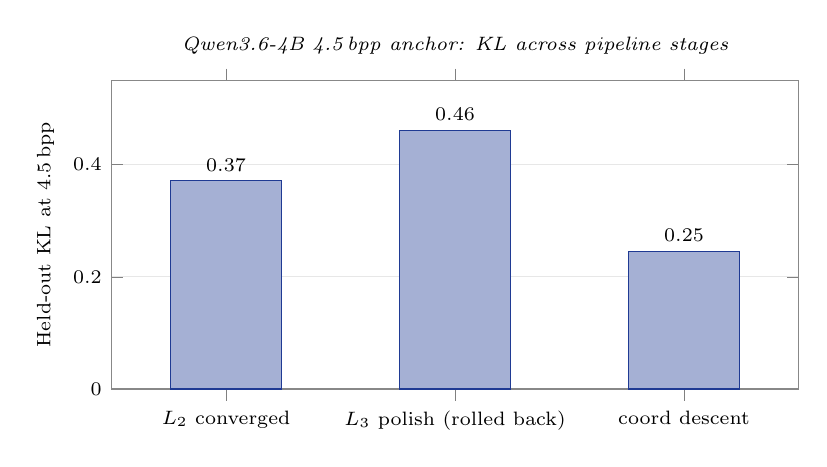
\begin{tikzpicture}
\begin{axis}[
  width=0.85\linewidth,
  height=5.5cm,
  ybar,
  bar width=14mm,
  ylabel={Held-out KL at 4.5\,bpp},
  symbolic x coords={$L_2$ converged, $L_3$ polish (rolled back), coord descent},
  xtick=data,
  ymin=0.0, ymax=0.55,
  ymajorgrids,
  major grid style={draw=rule!20},
  axis line style={draw=rule},
  tick label style={font=\scriptsize},
  label style={font=\scriptsize},
  title style={font=\scriptsize\itshape},
  title={Qwen3.6-4B 4.5\,bpp anchor: KL across pipeline stages},
  nodes near coords,
  nodes near coords style={font=\scriptsize},
  enlarge x limits=0.25
]
\addplot[draw=accent, fill=accent!40] coordinates {
  ($L_2$ converged, 0.371)
  ($L_3$ polish (rolled back), 0.461)
  (coord descent, 0.245)
};
\end{axis}
\end{tikzpicture}
\caption{Pipeline progression at the Qwen3.6-4B 4.5\,bpp anchor.
$L_2$ converges to KL $0.371$. The $L_3$ polish DP applies the additive-DP
non-additivity bug at scale and \emph{regresses} to KL $0.461$ ($+24\%$);
the real-KL gate detects the regression and rolls the polish output
back to the prior assignment. Coord descent then commits 6 single-Linear
flips of 101 attempted, each gated on real held-out KL, ending at KL
$0.245$ ($-34\%$ versus $L_2$). The pattern is reproducible across every
4B anchor we have measured and is the empirical motivation for separating
candidate generation from candidate selection.}
\label{fig:4b_progression}
\end{figure}


The $L_3$ polish stage \emph{regresses} relative to $L_2$ ($0.371 \to 0.461$,
$+24\%$), consistent with the additive overshoot mechanism described in
Section~\ref{sec:theory}; the regression is detected by the real-KL gate
and the polish output is rolled back. The coordinate-descent stage
recovers and surpasses both: $0.461 \to 0.245$, with 6 flips committed out
of 101 attempts. The shipped 4B artifact at this anchor is the
coord-descent output. The same pattern reproduces at every Qwen-4B anchor we
have measured.

\subsection{Qwen3.6-27B production}\label{subsec:27b_results}

The Qwen3.6-27B PrismaSCOUT artifact (DOI \texttt{10.57967/hf/8656},
\cite{Tand2026hf}) is produced from the same source weights and
the same per-tensor toolkit
(GPTQ damp sweep, scale sweep, block-output match) as the previously
shipped \textsc{PrismaQuant}~v1 5.5~bpp artifact \cite{Tand2026hf_prev}. Only
the selection routine changed. Both artifacts are the empirical operating
point each selection regime deployed: $5.5$~bpp was where v1's
sensitivity-driven allocation, run under the same per-tensor toolkit,
produced the model that v1 deemed worth shipping; $5.31$~bpp is
PrismaSCOUT's validated-frontier kneedle (Section~\ref{subsec:kneedle}).
The head-to-head therefore measures what happens when the selection
regime changes around a fixed candidate-generation pipeline, not what
happens when the budget is held fixed and one asks which regime
quantizes better at that bpp.

\begin{table}[h]
\centering
\caption{Qwen3.6-27B: previously shipped \textsc{PrismaQuant}~v1 vs.\ current
  \textsc{PrismaSCOUT} artifact, same source weights and same per-tensor
  toolkit. Held-out KL on disjoint validation split, 8 samples
  $\times$ 512 tokens.}
\label{tab:27b_headline}
\begin{tabular}{lrrr}
\toprule
Artifact & Size & bpp & Held-out KL \\
\midrule
\textsc{PrismaQuant}~v1 (5.50 bpp) & 22.67 GB & 5.50 & 0.0475 \\
\textsc{PrismaSCOUT} (5.31 bpp)    & 20.17 GB & 5.31 & 0.0151 \\
\midrule
Change                              & $-2.5$ GB ($-11\%$) & $-0.19$ & $-0.0324$ ($-68\%$) \\
\bottomrule
\end{tabular}
\end{table}

The artifact is 11\% smaller and the held-out KL is $\sim 3.2\times$ lower.
The validated-frontier picture (Figure~\ref{fig:validated_27b}) is the
algorithmic explanation: the surrogate-only kneedle on the same candidate
set picks 5.857~bpp / KL~0.056; the validated kneedle picks 5.31~bpp /
KL~0.015. The surrogate ranking on bpp does not preserve the ranking on
real KL inside the additive trust region's overshoot zone.

\begin{figure}[t]
\centering
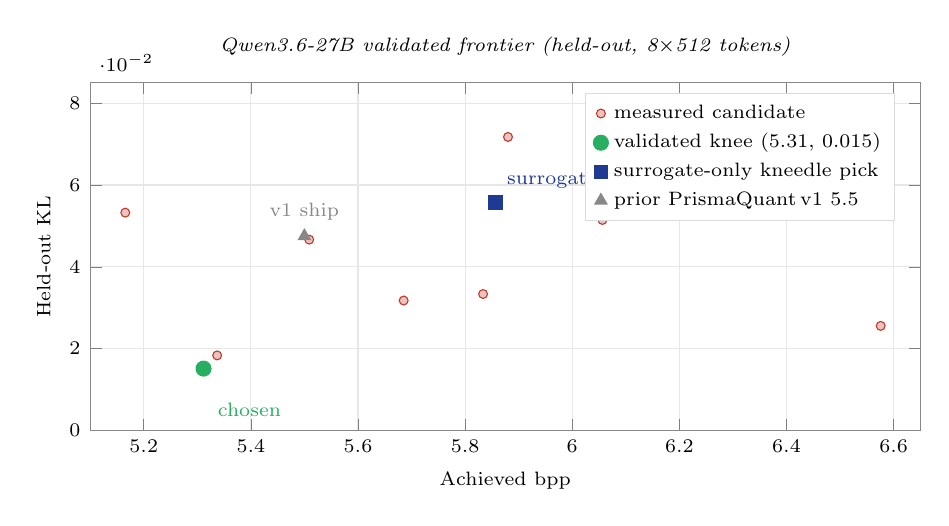
\begin{tikzpicture}
\begin{axis}[
  width=\linewidth,
  height=6.0cm,
  xlabel={Achieved $\bpp$},
  ylabel={Held-out KL},
  xmin=5.10, xmax=6.65,
  ymin=0.0, ymax=0.085,
  grid=both,
  major grid style={draw=rule!20},
  minor grid style={draw=rule!10},
  axis line style={draw=rule},
  tick label style={font=\scriptsize},
  label style={font=\scriptsize},
  title style={font=\scriptsize\itshape},
  title={Qwen3.6-27B validated frontier (held-out, 8$\times$512 tokens)},
  legend style={font=\scriptsize, draw=rule!30, fill=white, at={(0.97,0.97)}, anchor=north east},
  legend cell align={left}
]
% Validated points (achieved_bpp, validation_kl) from the 27B run
\addplot[
  only marks, mark=*, mark size=1.6pt,
  color=accent2, fill=accent2!30
]
table[row sep=\\] {
x  y  \\
5.1656 0.053241 \\
5.3117 0.015128 \\
5.3371 0.018352 \\
5.5090 0.046646 \\
5.6853 0.031769 \\
5.8336 0.033356 \\
5.8569 0.055692 \\
5.8801 0.071730 \\
6.0564 0.051443 \\
6.2280 0.075630 \\
6.4043 0.052859 \\
6.5759 0.025567 \\
};
\addlegendentry{measured candidate}

% Validated knee (5.31)
\addplot[
  only marks, mark=*, mark size=2.7pt,
  color=accent3
] coordinates {(5.3117, 0.015128)};
\addlegendentry{validated knee (5.31, 0.015)}

% Surrogate-only knee pick (5.857)
\addplot[
  only marks, mark=square*, mark size=2.4pt,
  color=accent
] coordinates {(5.8569, 0.055692)};
\addlegendentry{surrogate-only kneedle pick}

% Annotation for shipped 5.5
\addplot[
  only marks, mark=triangle*, mark size=2.5pt,
  color=rule
] coordinates {(5.5, 0.0475)};
\addlegendentry{prior PrismaQuant\,v1 5.5}

\node[font=\scriptsize, text=accent3, anchor=west] at (axis cs:5.32,0.005) {chosen};
\node[font=\scriptsize, text=accent, anchor=west] at (axis cs:5.86,0.061) {surrogate};
\node[font=\scriptsize, text=rule, anchor=south] at (axis cs:5.5,0.049) {v1 ship};

\end{axis}
\end{tikzpicture}
\caption{Validated-frontier candidates measured on the held-out validation
split for Qwen3.6-27B. Red filled circles are measured candidate
assignments. The surrogate-only kneedle on the same candidate set picks
$5.857$\,bpp at KL $0.056$ (dark-blue square). The validated kneedle
picks the dominating point at $5.3117$\,bpp / KL $0.0151$ (green disk,
shipped artifact); note the lower-bpp point at $5.166$ has higher
KL and is therefore $\eta$-dominated. The previously shipped
\textsc{PrismaQuant}~v1 artifact at $5.50$\,bpp / KL $0.0475$ (gray
triangle) sits inside the validated frontier --- the new selector finds a
strictly better point at lower bpp.}
\label{fig:validated_27b}
\end{figure}


\subsection{Downstream evaluation}

We report the downstream evaluation on the 27B PrismaSCOUT artifact in
Table~\ref{tab:27b_evals}. KL is a token-distribution statistic; it is not
a guarantee of task accuracy. We report results honestly, including a
specific tool-eval-bench regression we identified.

\begin{table}[h]
\centering
\caption{Qwen3.6-27B downstream evaluation under matched vLLM serve flags.
  Both artifacts served identically (\texttt{compressed-tensors},
  \texttt{kv-cache-dtype=fp8}, \texttt{enable-prefix-caching}). Validator
  uses an internal $583$-token prompt suite. tool-eval-bench is
  reported separately at two scopes: the full hardmode suite (single trial,
  148 points) and a 10-scenario adversarial subset run with 3 trials each
  (20 points/trial). Both tool-eval invocations used \texttt{--no-think}
  and \texttt{--temperature 0}.}
\label{tab:27b_evals}
\footnotesize
\setlength{\tabcolsep}{4pt}
\begin{tabular}{lrrr}
\toprule
Metric & PrismaSCOUT (5.31) & PrismaQuant v1 (5.50) & $\Delta$ \\
\midrule
Held-out KL ($\downarrow$, $8\times 512$ tokens)  & \textbf{0.0151}   & 0.0475   & $-0.0324$ ($-68\%$) \\
GSM8K strict ($\uparrow$)                          & 96.66\%           & \textbf{96.74\%} & $-0.08$ pp \\
GSM8K flexible ($\uparrow$)                        & 96.59\%           & \textbf{96.66\%} & $-0.08$ pp \\
IFEval prompt strict ($\uparrow$)                  & \textbf{85.40\%}  & 84.66\%  & $+0.74$ pp \\
IFEval prompt loose ($\uparrow$)                   & \textbf{88.72\%}  & 87.80\%  & $+0.92$ pp \\
IFEval instruction strict ($\uparrow$)             & \textbf{89.93\%}  & 89.81\%  & $+0.12$ pp \\
IFEval instruction loose ($\uparrow$)              & \textbf{92.45\%}  & 92.09\%  & $+0.36$ pp \\
MMLU 5-shot (limit $20$ / subj.) ($\uparrow$)      & 86.23\%           & \textbf{87.19\%} & $-0.96$ pp \\
Validator perplexity ($\downarrow$)                & \textbf{4.128}    & 4.178    & $-0.050$ \\
Validator mean NLL ($\downarrow$)                  & \textbf{1.4178}   & 1.4297   & $-0.012$ \\
Validator max prompt-avg NLL ($\downarrow$)        & 1.8946            & \textbf{1.8350} & $+0.060$ \\
\midrule
\multicolumn{4}{l}{\emph{tool-eval-bench, full hardmode sequential suite (single trial, 148 pts)}} \\
\quad final score ($\uparrow$)                     & \textbf{88/100}   & 85/100   & $+3$ \\
\quad total points ($\uparrow$)                    & \textbf{130/148}  & 126/148  & $+4$ \\
\quad safety-critical failures ($\downarrow$)      & 4                 & \textbf{3} & $+1$ \\
\midrule
\multicolumn{4}{l}{\emph{tool-eval-bench, targeted adversarial subset (10 scenarios $\times$ 3 trials, 20 pts)}} \\
\quad mean final score ($\uparrow$)                & \textbf{30/100}   & 25/100   & $+5$ \\
\quad mean points ($\uparrow$)                     & \textbf{6.0/20}   & 5.0/20   & $+1.0$ \\
\quad pass@3 ($\uparrow$)                          & 10\%              & \textbf{20\%} & $-10$ pp \\
\quad safety warnings/trial ($\downarrow$)         & 4                 & \textbf{3} & $+1$ \\
\bottomrule
\end{tabular}
\end{table}

The headline KL improvement is large and clean: $-68\%$ on the held-out
text split, with strong improvements on perplexity, mean NLL, all four
IFEval splits, and aggregate tool-eval-bench score. But the comparison is
not uniformly favorable. PrismaSCOUT regresses by $0.96$ pp on MMLU
$5$-shot and is statistically tied on GSM8K ($\pm 0.08$ pp). The
validator \emph{max prompt-avg NLL} is also worse on 5.31 ($1.8946$
vs.\ $1.8350$), indicating that the lower \emph{mean} KL is accompanied
by a heavier tail. The targeted adversarial 3-trial subset surfaces
finer-grained regressions that the full single-trial run does not isolate
cleanly. Scenario \texttt{TC-42} (extra-parameter injection in tool
calls) is a stable regression on $5.31$ (FAIL across all three trials)
where $5.5$ stably PASSES, and \texttt{TC-50} similarly degrades from
PASS to PARTIAL. Both artifacts share a vulnerability to \texttt{TC-60}
(cross-turn sleeper injection); both follow an attacker BCC inserted
via a tool result. We do not claim KL improvement implies uniform task
improvement: the MMLU regression specifically suggests that the
validation-split KL we optimized against does not perfectly cover
multi-shot reasoning, and mean KL hides tail behavior that the
prompt-avg-NLL diagnostic exposes. Future work includes p95/p99 KL
diagnostics, a schema-focused KL gate, and an MMLU-style multi-shot
calibration slice (Section~\ref{sec:discussion}). The benchmark numbers
above are reproduced verbatim from the model card at
DOI~\texttt{10.57967/hf/8656} \cite{Tand2026hf}.

\subsection{Production-faithful polish on Qwen3.6-27B}\label{subsec:prodpolish_results}

Section~\ref{subsec:prodpolish} described the production-faithful polish:
delta-quantize \texttt{WeightSession} swaps one decision unit's weight in
place per trial, weights are rendered through a closer approximation of
the export pipeline (GPTQ, scale-sweep, joint sibling-coherent NVFP4
input global scales, calibrated activation clip; block-output match,
remains on the export-only side and is not yet replicated in the
polish-time evaluator), and the move set is a
single bottom-up sweep from a low-bpp floor under a $5\%$ bits-budget
creep. Table~\ref{tab:27b_prodpolish} reports the polish-time KL outcome
on Qwen3.6-27B; both rows are evaluated on the same matched
$2\!\times\!128$ token calibration that the upstream PrismaSCOUT
selection used during its kneedle search. This is a polish-time signal,
not a held-out claim --- a re-measurement on the larger
$8\!\times\!512$ split that backs the v1 5.5~bpp baseline is in flight.

\begin{table}[h]
\centering
\caption{Qwen3.6-27B: production-faithful polish vs.\ shipped
  PrismaSCOUT, polish-time KL on a matched $2\!\times\!128$ token
  calibration set. Both rows use identical source weights and identical
  per-tensor toolkit; the polish operates on the same Block-CLADO
  decision units that PrismaSCOUT's surrogate hierarchy used.
  Calibration-matched but small; treat as polish-time signal pending
  $8\!\times\!512$ re-measurement.}
\label{tab:27b_prodpolish}
\begin{tabular}{lrrr}
\toprule
Artifact & bpp & Polish-time KL ($2{\times}128$) & Relative \\
\midrule
\textsc{PrismaSCOUT} (5.31)             & 5.31           & 0.0151          & --- \\
Production-faithful polish (5.39)       & \textbf{5.39}  & \textbf{0.0054} & $-2.8\times$ at $+0.08$ bpp (provisional) \\
\bottomrule
\end{tabular}
\end{table}

The polish committed $12$ accepted moves in $28$ minutes wall on a single
GB10 (delta-quantize \texttt{WeightSession} with disk-streaming
\texttt{ProductionWeightCache} and a 5~GiB LRU bound). Per-Linear, the
disagreement with PrismaSCOUT's assignment is large
(Table~\ref{tab:27b_prodpolish_diff}): $144$ of $497$ language-domain
Linears change format, with the new assignment concentrating its
high-precision budget on a tight set of bottleneck Linears.

\begin{table}[h]
\centering
\caption{Per-Linear format disagreement on the $497$-entry language-domain
  assignment between PrismaSCOUT (5.31~bpp) and the production-faithful
  polish (5.39~bpp). Disagreement total: $144/497 = 29.0\%$.}
\label{tab:27b_prodpolish_diff}
\begin{tabular}{lr}
\toprule
PrismaSCOUT $\to$ polish & \# Linears \\
\midrule
BF16  $\to$ NVFP4   & 132 \\
NVFP4 $\to$ BF16    & 8 \\
NVFP4 $\to$ MXFP8   & 3 \\
BF16  $\to$ MXFP8   & 1 \\
\midrule
By role: \texttt{linear\_attn} & 104/240 (43\%) \\
\quad\phantom{By role:} \texttt{self\_attn}   & 31/64 (48\%) \\
\quad\phantom{By role:} \texttt{mlp}          & 9/192 (5\%) \\
\bottomrule
\end{tabular}
\end{table}

The structural finding is that PrismaSCOUT's surrogate hierarchy spent its
high-precision budget distributively --- $132$ of $137$ BF16 picks were
small \texttt{linear\_attn.in\_proj\_\{a, b\}} rank-projection matrices,
which a per-element saliency surrogate flags as gradient-sensitive. Real
KL on production-faithful weights judges these matrices cheap to quantize
to NVFP4 and reclaims their bit budget for a much smaller set of expensive
Linears: \texttt{mlp.down\_proj} at layers $\{0, 10, 16, 62\}$,
\texttt{mlp.\{gate, up\}\_proj} at $\{16, 19\}$, the embedding-adjacent
layer-$0$ \texttt{linear\_attn} block, layer-$24$ \texttt{out\_proj}, and
layer-$32$ \texttt{in\_proj\_\{qkv, z\}}. PrismaSCOUT's single MXFP8 pick
(\texttt{layer 14 linear\_attn.out\_proj}) is the only one that survives
into the polish; the polish adds four new MXFP8 picks at
$\{1, 16, 19_a, 19_b\}$.

The polish's KL improvement does not yet have downstream task numbers
attached: the export of the $5.39$~bpp artifact and the matched-flag
serve-time evaluation suite (validator perplexity, GSM8K, IFEval, MMLU,
tool-eval-bench) are in flight at the time of writing. The held-out KL is
the conservative claim --- the same statistic that selected the
PrismaSCOUT~$5.31$~bpp artifact in the first place. Whether the
$2.8\times$ KL drop translates into the downstream improvements
Section~\ref{subsec:27b_results} reported for the surrogate
$\to$ validated-frontier upgrade, or surfaces fresh tail regressions of
its own, remains an open question we will report when the eval suite
completes.

A first run of the production-faithful polish reported a final
\texttt{bpp} below the all-NVFP4 floor due to a key mismatch in an
ad-hoc payload writer: it serialized decision-unit members under
\texttt{member\_qnames} but \texttt{block\_clado.parse\_payload}
only recognized \texttt{members} and silently fell back to a singleton
pseudo-member. Move-set fidelity is independently load-bearing of
cost-model fidelity: a silent fallback that turns expensive flips into
no-ops looks indistinguishable from a polish that converged fast. The
fix accepts both keys and \texttt{coord\_descent\_polish} now raises if
any decision unit has any member missing from the starting assignment.

\section{Discussion and Limitations}\label{sec:discussion}

\paragraph{Non-additivity is structural, not pathological.} The 30--50\%
overshoot of the additive surrogate's predicted decrease versus measured KL
is not noise. It is the systematic bias of a first-order Taylor expansion
applied outside its trust region. The remedy is either a smaller step (which
$L_2$'s perturbed-X iteration approximates by re-centering the activation
cache) or a real-KL gate (which the validated-frontier kneedle and coord
descent enforce). The shipping path uses both.

\paragraph{The kneedle is a model-selection criterion.} The kneedle is not a
universal optimum. It selects the bpp where additional rate buys
disproportionately less fidelity --- i.e., where the marginal cost of further
size reduction is high. It is the right shipping criterion under the implicit
loss
$\mathcal{L}(\bpp,\,\mathrm{KL}) = \alpha\cdot\mathrm{KL} + \beta\cdot\bpp$
with $\alpha,\beta$ proportional to the perpendicular axis weights, and a
reasonable default in the absence of an explicit task-cost-of-bits curve.
Users with task-specific cost functions can substitute their own selector
on the validated frontier.

\paragraph{The held-out KL is a calibration-set statistic.} The downstream
evaluation in Section~\ref{subsec:27b_results} confirms that lower held-out
KL does not entail uniform task improvement. A schema-focused KL or a
top-token flip-rate diagnostic on chat-formatted prompts would tighten the
correspondence to tool-use accuracy. We report the KL we measured and flag
the gaps.

\paragraph{Hardware-bounded measurement.} The cost hierarchy is calibrated
to fit in a 128~GB UMA host; on larger hosts, $L_3$ candidate budgets and
coord-descent pass counts can be substantially larger, and the Pareto
sweep can target denser frontiers. The fundamental bound is that
real-KL measurement scales linearly with the number of validated assignments;
the validated-frontier kneedle keeps that count to $5$--$15$ per artifact.

\paragraph{Limitations.}
(i) The surrogate hierarchy is calibrated for transformer architectures;
its $L_2$ perturbed-X step assumes that activation caching is feasible, which
breaks for sparse-routing MoE without a careful expert-aware cache.
(ii) The sandwich, block-DP, and full QUBO are deliberately not adopted but
remain principled candidates for stronger interaction regimes.
(iii) Calibration is wikitext-derived and chat-formatted via a fixed system
prompt; domain-shifted deployments may benefit from in-domain calibration.
(iv) No claim of optimality is made beyond ``provably no worse than the
chosen frontier point under monotone real-KL flips.'' The frontier itself is
sampled, not exhaustive.

\section{Conclusion}

We described \textsc{PrismaQuant} and its core search algorithm
\textsc{PrismaSCOUT}: a mixed-precision LLM quantization pipeline whose
defining choice is to use surrogate cost models for candidate generation
only and to make every shipping decision on a real, end-to-end
Kullback--Leibler divergence measurement against a held-out calibration
split. The key engineering challenge was making that measurement loop
tractable on a 128~GB UMA host through a multi-level cost hierarchy with
lane-batched, tail-amortized $L_3$, validated-frontier kneedle selection
with a noise-floor dominance filter and leave-one-out stability, and a
monotone coord-descent polish that is provably non-regressive on real KL.

The shipping artifact on Qwen3.6-27B is 11\% smaller and 68\% lower in
held-out KL than the previously shipped \textsc{PrismaQuant}~v1 artifact at
the same source. A subsequent production-faithful polish, in which the
polish-time evaluator is upgraded to render a closer approximation of
the per-Linear quantized weights the exporter ships and the move set is
restructured around a low-bpp floor, drops the polish-time KL on the
same calibration from $0.0151$ to $0.0054$ at $+0.08$ bpp ($5.39$~bpp),
reclaiming the rank-projection bit budget that distributed-saliency
surrogates over-protect and concentrating it on a handful of
\texttt{mlp.down\_proj} bottleneck Linears. The polish-time signal still
needs to be re-measured on the larger validation calibration that backs
the v1 shipping baseline before becoming a load-bearing claim.
We also documented several principled numerical methods
(Lagrangian $\lambda$-bisection, sandwich proximal recalibration, block-DP
over architectural cliques, sparse pairwise QUBO, top-$K$ Hessian covering,
surrogate-only knee, probe-only knee predictor) that were considered during
design and either deprecated, made experimental-only, or rejected outright.
Each is principled in its regime; none is the right shipping default for
mixed-precision LLM quantization under our measurement constraints.

\paragraph{Reproduction.} The Qwen3.6-27B PrismaSCOUT artifact is available at
\url{https://huggingface.co/rdtand/Qwen3.6-27B-PrismaSCOUT-Blackwell-NVFP4-BF16-vllm}
(DOI \texttt{10.57967/hf/8656}, \cite{Tand2026hf}). The pipeline is open
source at \url{https://github.com/RobTand/prismaquant}; commits referenced
throughout (\texttt{8e503a5}, \texttt{2e670b3}, \texttt{444bc28}, \dots) are
visible there.

\section*{Acknowledgments}

The author acknowledges substantive technical consultation with several
large language model assistants during the design, implementation, and
review phases of this work, including the mathematical analysis of the
alternatives surveyed in Section~\ref{sec:rejected}. Deliberation
transcripts where the consultation was load-bearing for the paper's
narrative are preserved in \texttt{scratch/deliberation/} of the source
repository for audit.

\renewcommand{\refname}{References}

\begin{thebibliography}{99}

\bibitem{Tand2026hf} R.~Tand. \emph{Qwen3.6-27B-PrismaSCOUT-Blackwell-NVFP4-BF16-vllm.}
  Hugging Face model artifact, 2026. DOI: \texttt{10.57967/hf/8656}.
  \url{https://huggingface.co/rdtand/Qwen3.6-27B-PrismaSCOUT-Blackwell-NVFP4-BF16-vllm}.

\bibitem{Tand2026hf_prev} R.~Tand. \emph{Qwen3.6-27B-PrismaQuant-5.5bit-vllm.}
  Hugging Face model artifact, 2026.
  \url{https://huggingface.co/rdtand/Qwen3.6-27B-PrismaQuant-5.5bit-vllm}.

\bibitem{prismaquant} R.~Tand. \emph{PrismaQuant: per-Linear sensitivity-driven
  mixed-precision quantization for LLMs.}
  \url{https://github.com/RobTand/prismaquant}, 2026.

\bibitem{gptq2022} E.~Frantar, S.~Ashkboos, T.~Hoefler, and D.~Alistarh. GPTQ:
  Accurate post-training quantization for generative pre-trained transformers.
  \emph{ICLR}, 2023. \url{https://arxiv.org/abs/2210.17323}.

\bibitem{autoround2023} W.~Cheng, Y.~Lv, W.~Zhang, and H.~Shen. Optimize weight
  rounding via signed gradient descent for the quantization of LLMs.
  \emph{arXiv:2309.05516}, 2023.

\bibitem{hawqv3} Z.~Yao, Z.~Dong, Z.~Zheng, A.~Gholami, J.~Yu, E.~Tan, L.~Wang,
  Q.~Huang, Y.~Wang, M.~W.~Mahoney, and K.~Keutzer.
  HAWQ-V3: Dyadic Neural Network Quantization. \emph{ICML}, 2021.
  arXiv:2011.10680.

\bibitem{clado2023} Z.~Deng, S.~Sharify, X.~Wang, and M.~Orshansky.
  Mixed-Precision Quantization for Deep Vision Models with Integer
  Quadratic Programming (CLADO: Cross-LAyer-Dependency-aware
  Optimization). \emph{Proceedings of the 62nd Annual Design
  Automation Conference (DAC)}, 2025. arXiv:2307.05657.

\bibitem{coopq} J.~Zhao, A.~Derakhshan, J.~Kana~Hyman, J.~Dong,
  S.~Abdu~Jyothi, and I.~Harris. CoopQ: Cooperative Game Inspired Layerwise
  Mixed Precision Quantization for LLMs. \emph{arXiv:2509.15455}, 2025.

\bibitem{amq} S.~Lee, S.-T.~Woo, J.~Jin, C.~Lee, and E.~Park. AMQ: Enabling
  AutoML for Mixed-precision Weight-Only Quantization of Large Language
  Models. \emph{arXiv:2509.12019}, 2025.

\bibitem{mpq_survey} M.~Rakka, M.~Fournarakis, O.~Krestinskaya, J.~Bazzi,
  K.~N.~Salama, F.~Kurdahi, A.~M.~Eltawil, and M.~E.~Fouda.
  Mixed-Precision Quantization for Language Models: Techniques and
  Prospects. \emph{arXiv:2510.16805}, 2025.

\bibitem{iterquant2026} H.~Jeong, J.~Kim, H.~Kwon, J.~Lee, and Y.~Lee.
  IterQuant: Iterative Quantization Framework for Mixed-Precision LLM
  Compression. \emph{DATE}, 2026.

\bibitem{geometry_aware} J.~Chen, Y.~Shabanzadeh, E.~Crn{\v c}evi{\'c},
  T.~Hoefler, and D.~Alistarh. The Geometry of LLM Quantization: GPTQ as
  Babai's Nearest Plane Algorithm. \emph{ICLR}, 2026. arXiv:2507.18553.

\bibitem{paroquant} Y.~Liang, H.~Chen, Z.~Zhang, S.~Han, and Z.~Liu.
  ParoQuant: Pairwise Rotation Quantization for Efficient Reasoning LLM
  Inference. \emph{ICLR}, 2026. arXiv:2511.10645.

\bibitem{kneedle2011} V.~Satopaa, J.~Albrecht, D.~Irwin, and B.~Raghavan.
  Finding a ``Kneedle'' in a Haystack: Detecting Knee Points in System
  Behavior. In \emph{31st International Conference on Distributed
  Computing Systems Workshops (ICDCSW)}, pages 166--171, 2011.

\bibitem{ortega1998} A.~Ortega and K.~Ramchandran. Rate-Distortion Methods
  for Image and Video Compression. \emph{IEEE Signal Processing Magazine},
  15(6):23--50, 1998.

\bibitem{ocp_mx} Open Compute Project. \emph{OCP Microscaling Formats (MX)
  Specification, Version 1.0.} OCP, September 2023.
  \url{https://www.opencompute.org/documents/ocp-microscaling-formats-mx-v1-0-spec-final-pdf}.

\bibitem{nvfp4_blackwell} NVIDIA Corporation. \emph{NVIDIA Blackwell
  Architecture and the NVFP4 Format.} NVIDIA Technical Briefs, 2024--2025.

\bibitem{vllm} W.~Kwon, Z.~Li, S.~Zhuang, Y.~Sheng, L.~Zheng, C.~H.~Yu,
  J.~Gonzalez, H.~Zhang, and I.~Stoica. Efficient Memory Management for
  Large Language Model Serving with PagedAttention. In \emph{Proceedings
  of the 29th Symposium on Operating Systems Principles (SOSP)}, 2023.

\bibitem{shapley_potential_games} D.~Monderer and L.~Shapley. Potential
  Games. \emph{Games and Economic Behavior}, 14(1):124--143, 1996.

\end{thebibliography}

\appendix

\section{Fused-sibling aggregation}\label{app:fused}

Fused siblings in attention ($q,k,v$) and MoE ($\mathrm{gate\_up}$,
$\mathrm{down}$) must share one format choice in vLLM's fused kernel. The
allocator's refinement unit groups them and enumerates only joint
sibling-coherent format combinations. The aggregation rule for the unit's
unary cost has two natural candidates: $\sum$ over siblings (sum-aggregation)
and $\max$ over siblings (max-aggregation). Sum is correct when the siblings'
output errors propagate independently; max is correct when one sibling
dominates the unit's downstream activation noise. Empirically on
Qwen3.6-27B, sum-aggregation matches the measured $L_3$ end-KL more closely
on both attention and MoE units (commit \texttt{d370c3e}, ``allocator: revert
to sum-aggregation for fused siblings (right thing on principle)''). We use
sum.

\section{Allocator runtime parameters}

Defaults below are taken from the argument parser of
\texttt{prismaquant.iterate\_perturbed\_allocation} at the
audit-consensus commit (\texttt{2e670b3}).

\begin{itemize}[leftmargin=*]
  \item $L_2$: \texttt{bit\_precision}~$=0.001$, \texttt{convergence-frac}
    (weighted-Hamming flip ratio)~$=0.01$, \texttt{max-iters}~$=5$,
    \texttt{ema-decay}~$=0.5$, \texttt{n-calib-samples}~$=8$,
    \texttt{input-rows}~$=256$.
  \item $L_3$:
    \texttt{l3-uncertainty-rel-tol}~$=0.10$,
    \texttt{l3-min-fraction}~$=0.05$,
    \texttt{l3-max-fraction}~$=0.30$,
    \texttt{l3-safety-fraction}~$=0.02$,
    \texttt{l3-max-lanes-per-batch}~$=64$ (UMA-cap aware),
    \texttt{l3-tail-only}~$=$~on,
    \texttt{l3-regression-tolerance}~$=0.0$.
  \item Validated-frontier kneedle:
    \texttt{DEFAULT\_KNEE\_KL\_NOISE\_FLOOR} $\eta = 1\times 10^{-5}$,
    bisection tolerance \texttt{knee-tolerance}~$=0.05$ bpp,
    leave-one-out diagnostic engaged at $\ge 4$ frontier points,
    instability fallback policy \texttt{best-kl} (replaces the geometric
    knee with the lowest-KL frontier point).
  \item Coord descent: \texttt{max-passes}~$=1$,
    \texttt{early-stop-streak}~$=50$,
    \texttt{max-lanes-per-batch}~$=64$.
\end{itemize}

\section{Reproduction manifest for the Qwen3.6-27B PrismaSCOUT artifact}\label{app:repro}

The following pointers are sufficient to retrace the production 27B run
end-to-end. The artifact itself is at DOI \texttt{10.57967/hf/8656},
\cite{Tand2026hf}.

\begin{itemize}[leftmargin=*]
  \item \textbf{Pipeline source:} \url{https://github.com/RobTand/prismaquant},
    audit-consensus commit \texttt{2e670b3} (\emph{Implement PR-Polish-1:
    Rename validation\_kl and secure surrogate knee}). The kneedle search,
    archive DP, and L3 polish reside in
    \texttt{prismaquant/iterate\_perturbed\_allocation.py};
    L2 perturbed-X cache in \texttt{prismaquant/perturbed\_x\_cache.py};
    propagated-cost L3 in \texttt{prismaquant/propagated\_cost.py};
    additive multi-choice knapsack DP in
    \texttt{prismaquant/allocator\_solver.py}.
  \item \textbf{Source weights:} \texttt{Qwen/Qwen3.6-27B} (BF16, HF Hub),
    snapshot taken locally as \texttt{/hfcache/qwen36-27b-bf16}.
  \item \textbf{Calibration:} wikitext-derived prompts, chat-formatted under
    a fixed system template, hashed by
    \texttt{prismaquant.allocator.calibration\_data\_hash}. Splits:
    \texttt{l3\_calib\_split=train} (cost generation),
    \texttt{kl\_calib\_split=validation} (real-KL gate);
    selection-time KL evaluated on $8\!\times\!512$ tokens of the
    validation split.
  \item \textbf{Run directories.} The no-seed archive search lives under
    \path{/home/rob/dq-runs/qwen3p6-27b-smrf-overnight/} as
    \path{27b-knee-archive-beam4-refine-noseed-20260504T022551Z}; the
    export run that produced the shipped checkpoint is in the same
    parent as
    \path{27b-export-5p3095-kneedle-20260504T025719Z}. Matched-flag vLLM
    eval reports (\texttt{validate\_5p3095.md},
    \texttt{validate\_5p5.md}, tool-eval-bench summaries) live under that
    export run's \texttt{evals/} subtree.
  \item \textbf{Hardware:} NVIDIA GB10 Blackwell, 128~GB UMA; CUDA toolkit
    matched to the vLLM container (\texttt{vllm-fresh-b12x:latest}).
  \item \textbf{Serving:} vLLM with
    \texttt{-{}-quantization compressed-tensors -{}-kv-cache-dtype fp8
    -{}-enable-prefix-caching -{}-max-model-len 32768
    -{}-tool-call-parser qwen3\_coder}.
  \item \textbf{Determinism:} the run is reproducible up to floating-point
    determinism on the same Blackwell host. The full audit trail
    (validated-frontier candidates, dominance filter parameters, knee,
    leave-one-out shadow knees, coord-descent flip log, L2 iteration
    trace) is written to the run's \texttt{out/} directory.
\end{itemize}

\end{document}
